\documentclass{beamer}
\usetheme{AnnArbor}
\usecolortheme{spruce}
\usepackage{circuitikz}
\usepackage{graphicx}

\title{Multiplexers \& Demultiplexers}
\subtitle{Why use many wire when few wire do trick}
\author[A Praveen]{Akilesh Praveen - CMSC389E}
\institute{UMD}
\date{\today}



\begin{document}

    % title page
    \begin{frame}
        \titlepage
    \end{frame}
    
    % table of contents
    \begin{frame}
        \frametitle{Agenda}
        \tableofcontents
    \end{frame}
    
    \section{Announcements}
    
        \begin{frame}
                \vfill
                \centering
                \begin{beamercolorbox}[sep=8pt,center,shadow=true,rounded=true]{title}
                    \usebeamerfont{title}Announcements\par%
                \end{beamercolorbox}
                \vfill
             \end{frame}
    
        \subsection{Project 4}
        
            
            
            \begin{frame}
                \frametitle{Project 4}
                \begin{itemize}
                    \item Project 4's been released, and the name of the game is multipliers.
                    \item You'll find everything you need under the 'week 5' section on the course website
                    \item Today's lecture will give you background knowledge that will help you implement multiplexers and demultiplexers.
                    
                    \item More info to come at the end of lecture
                    
                \end{itemize}
            \end{frame}
            
    \section{Multiplexers \& Demultiplexers}
    
    	\subsection{Introduction}
    	
    	\begin{frame}
                \vfill
                \centering
                \begin{beamercolorbox}[sep=8pt,center,shadow=true,rounded=true]{title}
                    \usebeamerfont{title}Muxes and Demuxes\par%
                \end{beamercolorbox}
                \vfill
             \end{frame}
    	
    	
    	\begin{frame}
			\frametitle{An example}
      


\tikzset{every picture/.style={line width=0.75pt}} %set default line width to 0.75pt        

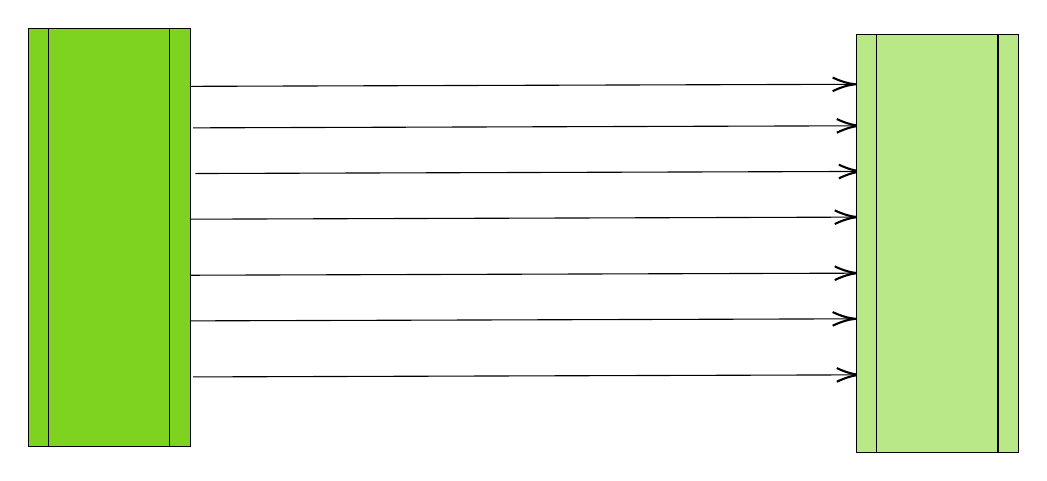
\begin{tikzpicture}[x=0.75pt,y=0.75pt,yscale=-1,xscale=1]
%uncomment if require: \path (0,300); %set diagram left start at 0, and has height of 300

%Straight Lines [id:da797417316267886] 
\draw    (98.5,64) -- (417.5,63.01) ;
\draw [shift={(419.5,63)}, rotate = 539.8199999999999] [color={rgb, 255:red, 0; green, 0; blue, 0 }  ][line width=0.75]    (10.93,-3.29) .. controls (6.95,-1.4) and (3.31,-0.3) .. (0,0) .. controls (3.31,0.3) and (6.95,1.4) .. (10.93,3.29)   ;
%Straight Lines [id:da9867161861578443] 
\draw    (100.5,84) -- (419.5,83.01) ;
\draw [shift={(421.5,83)}, rotate = 539.8199999999999] [color={rgb, 255:red, 0; green, 0; blue, 0 }  ][line width=0.75]    (10.93,-3.29) .. controls (6.95,-1.4) and (3.31,-0.3) .. (0,0) .. controls (3.31,0.3) and (6.95,1.4) .. (10.93,3.29)   ;
%Straight Lines [id:da17622714748979218] 
\draw    (101.5,106) -- (420.5,105.01) ;
\draw [shift={(422.5,105)}, rotate = 539.8199999999999] [color={rgb, 255:red, 0; green, 0; blue, 0 }  ][line width=0.75]    (10.93,-3.29) .. controls (6.95,-1.4) and (3.31,-0.3) .. (0,0) .. controls (3.31,0.3) and (6.95,1.4) .. (10.93,3.29)   ;
%Straight Lines [id:da3187699597458509] 
\draw    (99.5,128) -- (418.5,127.01) ;
\draw [shift={(420.5,127)}, rotate = 539.8199999999999] [color={rgb, 255:red, 0; green, 0; blue, 0 }  ][line width=0.75]    (10.93,-3.29) .. controls (6.95,-1.4) and (3.31,-0.3) .. (0,0) .. controls (3.31,0.3) and (6.95,1.4) .. (10.93,3.29)   ;
%Straight Lines [id:da5165041416753314] 
\draw    (99.5,155) -- (418.5,154.01) ;
\draw [shift={(420.5,154)}, rotate = 539.8199999999999] [color={rgb, 255:red, 0; green, 0; blue, 0 }  ][line width=0.75]    (10.93,-3.29) .. controls (6.95,-1.4) and (3.31,-0.3) .. (0,0) .. controls (3.31,0.3) and (6.95,1.4) .. (10.93,3.29)   ;
%Straight Lines [id:da10098087423079927] 
\draw    (98.5,177) -- (417.5,176.01) ;
\draw [shift={(419.5,176)}, rotate = 539.8199999999999] [color={rgb, 255:red, 0; green, 0; blue, 0 }  ][line width=0.75]    (10.93,-3.29) .. controls (6.95,-1.4) and (3.31,-0.3) .. (0,0) .. controls (3.31,0.3) and (6.95,1.4) .. (10.93,3.29)   ;
%Straight Lines [id:da14963118622609028] 
\draw    (100.5,204) -- (419.5,203.01) ;
\draw [shift={(421.5,203)}, rotate = 539.8199999999999] [color={rgb, 255:red, 0; green, 0; blue, 0 }  ][line width=0.75]    (10.93,-3.29) .. controls (6.95,-1.4) and (3.31,-0.3) .. (0,0) .. controls (3.31,0.3) and (6.95,1.4) .. (10.93,3.29)   ;
%Flowchart: Prodefined Process [id:dp12787585466953033] 
\draw  [fill={rgb, 255:red, 126; green, 211; blue, 33 }  ,fill opacity=1 ] (21,36) -- (99,36) -- (99,237.5) -- (21,237.5) -- cycle ; \draw   (30.75,36) -- (30.75,237.5) ; \draw   (89.25,36) -- (89.25,237.5) ;
%Flowchart: Prodefined Process [id:dp585559902263576] 
\draw  [fill={rgb, 255:red, 184; green, 233; blue, 134 }  ,fill opacity=1 ] (420,39) -- (498,39) -- (498,240.5) -- (420,240.5) -- cycle ; \draw   (429.75,39) -- (429.75,240.5) ; \draw   (488.25,39) -- (488.25,240.5) ;




\end{tikzpicture}


			\begin{itemize}
				\item We've started creating circuits that have a sizable amount of wires associated with them
				\item It turns out, extending \textbf{all} of these wires is pretty expensive and space-consuming, given just how many wires we have to build
			\end{itemize}
			
			
			

		\end{frame}	
		
		
		\begin{frame}
			\frametitle{Parallel Signals}
			\begin{itemize}
				\item This phenomenon is known as having many \textbf{parallel signals}.
				\item They use a ton of wires!
				\item I'm sure everyone is well aware of how much more effort it is to place one extra line of wires in Minecraft, which makes you wonder how much harder it is to do in real life
				\item If we're going to be extending these wires over long distances, are there more efficent ways to handle that many signals?
			\end{itemize}
		\end{frame}	
		
		\begin{frame}
			\frametitle{Parallel Signals}
			\begin{itemize}
				\item Yes!!!
				\item Your answer can be found in \textbf{Multiplexers} and \textbf{Demultiplexers}.
			\end{itemize}
		\end{frame}		
    	
    	\begin{frame}
    		\frametitle{Multiplexers \& Demultiplexers}
    		
    		\begin{itemize}
    			\item A \textbf{Multiplexer} is often called a 'mux'.
    			\item A \textbf{Demultiplexer} is often called a 'demux'.
    		\end{itemize}
    		
		\end{frame}  
		
		\begin{frame}
    		\frametitle{Multiplexers \& Demultiplexers}
    		
    		\begin{itemize}
    			\item A \textbf{Multiplexer} is often called a 'mux'.
    			\item A \textbf{Demultiplexer} is often called a 'demux'.
    			\item The question is- what are they?
    		\end{itemize}
    		
		\end{frame}
		
		\begin{frame}
			\frametitle{Need necessitates solution}
			\begin{itemize}
				\item The need for \textbf{Multiplexers} arose due to the presence of a certain problem in digital circuit design.
				\item Think back to our bus designs, and our encoders and decoders
				\item It turns out, there are a lot of different circuits that would require us to have a fair amount of parallel wires.
				\item In other words, it's a \textbf{common problem} in digital logic design to have to deal with a multitude of \textbf{parallel signals}.
				
			\end{itemize}
		\end{frame}		 
		
			  	        
        
    
    	\subsection{What are Muxes and Demuxes?}
    	
    	\begin{frame}
    		\frametitle{What are they?}
    		\begin{itemize}
    			\item A \textbf{Multiplexer}, or \textbf{Mux}, takes a bunch of parallel wires and condenses all of them down to a singular \texttt{OUT} wire and a few \texttt{SELECT} wires.
    			\item A \textbf{Demultiplexer}, or \textbf{Demux}, takes a singular \texttt{IN} wire and a few \texttt{SELECT} wires, and sends the \texttt{IN} signal down the appropriate output wire.
    		\end{itemize}
    	\end{frame}
    	
    	\begin{frame}
    		\frametitle{What are they?}
    		\begin{itemize}
    			\item A \textbf{Multiplexer}, or \textbf{Mux}, takes a bunch of parallel wires and condenses all of them down to a singular \texttt{OUT} wire and a few \texttt{SELECT} wires.
    			\item A \textbf{Demultiplexer}, or \textbf{Demux}, takes a singular \texttt{IN} wire and a few \texttt{SELECT} wires, and sends the \texttt{IN} signal down the appropriate output wire.
    		\end{itemize}
    		
    		
			

\tikzset{every picture/.style={line width=0.75pt}} %set default line width to 0.75pt        

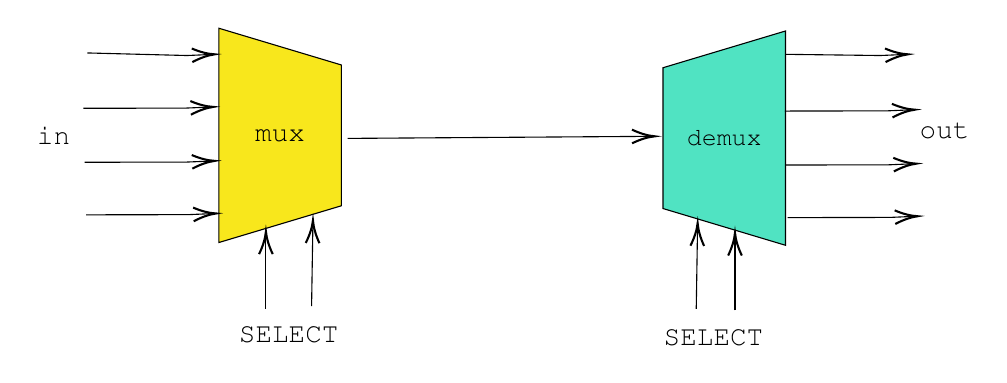
\begin{tikzpicture}[x=0.75pt,y=0.75pt,yscale=-1,xscale=1]
%uncomment if require: \path (0,300); %set diagram left start at 0, and has height of 300

%Shape: Trapezoid [id:dp9676716720394224] 
\draw  [fill={rgb, 255:red, 248; green, 231; blue, 28 }  ,fill opacity=1 ] (127,83.42) -- (186,101.12) -- (186,168.97) -- (127,186.67) -- cycle ;
%Shape: Trapezoid [id:dp8112150659093363] 
\draw  [fill={rgb, 255:red, 80; green, 227; blue, 194 }  ,fill opacity=1 ] (400,188) -- (341,170.3) -- (341,102.45) -- (400,84.75) -- cycle ;
%Straight Lines [id:da17513161874771777] 
\draw    (189,136.5) -- (335,135.51) ;
\draw [shift={(337,135.5)}, rotate = 539.61] [color={rgb, 255:red, 0; green, 0; blue, 0 }  ][line width=0.75]    (10.93,-3.29) .. controls (6.95,-1.4) and (3.31,-0.3) .. (0,0) .. controls (3.31,0.3) and (6.95,1.4) .. (10.93,3.29)   ;
%Straight Lines [id:da7314260725072124] 
\draw    (63.67,95.33) -- (111.64,96.57) -- (123,96.08) ;
\draw [shift={(125,96)}, rotate = 537.5699999999999] [color={rgb, 255:red, 0; green, 0; blue, 0 }  ][line width=0.75]    (10.93,-3.29) .. controls (6.95,-1.4) and (3.31,-0.3) .. (0,0) .. controls (3.31,0.3) and (6.95,1.4) .. (10.93,3.29)   ;
%Straight Lines [id:da32898600894177765] 
\draw    (61.67,122) -- (110.98,121.9) -- (122.34,121.42) ;
\draw [shift={(124.33,121.33)}, rotate = 537.5699999999999] [color={rgb, 255:red, 0; green, 0; blue, 0 }  ][line width=0.75]    (10.93,-3.29) .. controls (6.95,-1.4) and (3.31,-0.3) .. (0,0) .. controls (3.31,0.3) and (6.95,1.4) .. (10.93,3.29)   ;
%Straight Lines [id:da7983247275507934] 
\draw    (62.33,148) -- (111.64,147.9) -- (123,147.42) ;
\draw [shift={(125,147.33)}, rotate = 537.5699999999999] [color={rgb, 255:red, 0; green, 0; blue, 0 }  ][line width=0.75]    (10.93,-3.29) .. controls (6.95,-1.4) and (3.31,-0.3) .. (0,0) .. controls (3.31,0.3) and (6.95,1.4) .. (10.93,3.29)   ;
%Straight Lines [id:da04807653219902874] 
\draw    (63,173.33) -- (112.31,173.23) -- (123.67,172.75) ;
\draw [shift={(125.67,172.67)}, rotate = 537.5699999999999] [color={rgb, 255:red, 0; green, 0; blue, 0 }  ][line width=0.75]    (10.93,-3.29) .. controls (6.95,-1.4) and (3.31,-0.3) .. (0,0) .. controls (3.31,0.3) and (6.95,1.4) .. (10.93,3.29)   ;
%Straight Lines [id:da5159526044803394] 
\draw    (400.33,96) -- (445.64,96.57) -- (457,96.08) ;
\draw [shift={(459,96)}, rotate = 537.5699999999999] [color={rgb, 255:red, 0; green, 0; blue, 0 }  ][line width=0.75]    (10.93,-3.29) .. controls (6.95,-1.4) and (3.31,-0.3) .. (0,0) .. controls (3.31,0.3) and (6.95,1.4) .. (10.93,3.29)   ;
%Straight Lines [id:da8929745222846369] 
\draw    (399.67,123.33) -- (448.98,123.23) -- (460.34,122.75) ;
\draw [shift={(462.33,122.67)}, rotate = 537.5699999999999] [color={rgb, 255:red, 0; green, 0; blue, 0 }  ][line width=0.75]    (10.93,-3.29) .. controls (6.95,-1.4) and (3.31,-0.3) .. (0,0) .. controls (3.31,0.3) and (6.95,1.4) .. (10.93,3.29)   ;
%Straight Lines [id:da5083766804065095] 
\draw    (400.33,149.33) -- (449.64,149.23) -- (461,148.75) ;
\draw [shift={(463,148.67)}, rotate = 537.5699999999999] [color={rgb, 255:red, 0; green, 0; blue, 0 }  ][line width=0.75]    (10.93,-3.29) .. controls (6.95,-1.4) and (3.31,-0.3) .. (0,0) .. controls (3.31,0.3) and (6.95,1.4) .. (10.93,3.29)   ;
%Straight Lines [id:da4565821283716822] 
\draw    (401,174.67) -- (450.31,174.57) -- (461.67,174.08) ;
\draw [shift={(463.67,174)}, rotate = 537.5699999999999] [color={rgb, 255:red, 0; green, 0; blue, 0 }  ][line width=0.75]    (10.93,-3.29) .. controls (6.95,-1.4) and (3.31,-0.3) .. (0,0) .. controls (3.31,0.3) and (6.95,1.4) .. (10.93,3.29)   ;
%Straight Lines [id:da9657285985744374] 
\draw    (149.67,218.67) -- (149.67,183.33) ;
\draw [shift={(149.67,181.33)}, rotate = 450] [color={rgb, 255:red, 0; green, 0; blue, 0 }  ][line width=0.75]    (10.93,-3.29) .. controls (6.95,-1.4) and (3.31,-0.3) .. (0,0) .. controls (3.31,0.3) and (6.95,1.4) .. (10.93,3.29)   ;
%Straight Lines [id:da15318619740493855] 
\draw    (171.67,217.33) -- (172.3,178) ;
\draw [shift={(172.33,176)}, rotate = 450.92] [color={rgb, 255:red, 0; green, 0; blue, 0 }  ][line width=0.75]    (10.93,-3.29) .. controls (6.95,-1.4) and (3.31,-0.3) .. (0,0) .. controls (3.31,0.3) and (6.95,1.4) .. (10.93,3.29)   ;
%Straight Lines [id:da870193447515214] 
\draw    (375.67,219.33) -- (375.67,184) ;
\draw [shift={(375.67,182)}, rotate = 450] [color={rgb, 255:red, 0; green, 0; blue, 0 }  ][line width=0.75]    (10.93,-3.29) .. controls (6.95,-1.4) and (3.31,-0.3) .. (0,0) .. controls (3.31,0.3) and (6.95,1.4) .. (10.93,3.29)   ;
%Straight Lines [id:da69110814819773] 
\draw    (357,218.67) -- (357.63,179.33) ;
\draw [shift={(357.67,177.33)}, rotate = 450.92] [color={rgb, 255:red, 0; green, 0; blue, 0 }  ][line width=0.75]    (10.93,-3.29) .. controls (6.95,-1.4) and (3.31,-0.3) .. (0,0) .. controls (3.31,0.3) and (6.95,1.4) .. (10.93,3.29)   ;

% Text Node
\draw (160.67,231) node   [align=left] {{\fontfamily{pcr}\selectfont SELECT}};
% Text Node
\draw (365.33,232.33) node   [align=left] {{\fontfamily{pcr}\selectfont SELECT}};
% Text Node
\draw (47.33,135) node   [align=left] {{\fontfamily{pcr}\selectfont in}};
% Text Node
\draw (476.67,133) node   [align=left] {{\fontfamily{pcr}\selectfont out}};
% Text Node
\draw (156.5,135.04) node   [align=left] {{\fontfamily{pcr}\selectfont mux}};
% Text Node
\draw (370.5,136.38) node   [align=left] {{\fontfamily{pcr}\selectfont {\small demux}}};


\end{tikzpicture}


    	\end{frame}
    	
    	\begin{frame}
    		\frametitle{What can we observe?}
    		\begin{itemize}
    			\item In the earlier example, instead of having to carry 4 wires across the distance spanned by the mux and demux, we only needed the singular output wire and the selector wires
    			\item In other words, we only need to worry about carrying the wires highlighted in red across the distance spanned by the mux and demux
    		\end{itemize}
    		
    		

\tikzset{every picture/.style={line width=0.75pt}} %set default line width to 0.75pt        

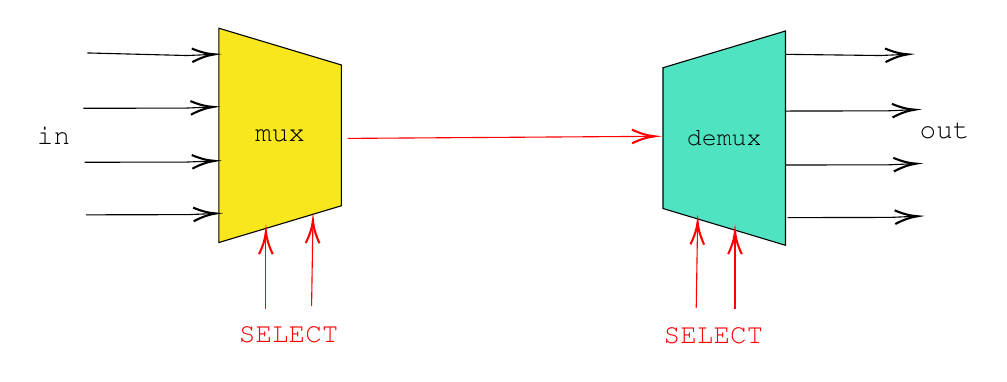
\begin{tikzpicture}[x=0.75pt,y=0.75pt,yscale=-1,xscale=1]
%uncomment if require: \path (0,300); %set diagram left start at 0, and has height of 300

%Shape: Trapezoid [id:dp9676716720394224] 
\draw  [fill={rgb, 255:red, 248; green, 231; blue, 28 }  ,fill opacity=1 ] (127,83.42) -- (186,101.12) -- (186,168.97) -- (127,186.67) -- cycle ;
%Shape: Trapezoid [id:dp8112150659093363] 
\draw  [fill={rgb, 255:red, 80; green, 227; blue, 194 }  ,fill opacity=1 ] (400,188) -- (341,170.3) -- (341,102.45) -- (400,84.75) -- cycle ;
%Straight Lines [id:da17513161874771777] 
\draw [color={rgb, 255:red, 255; green, 0; blue, 0 }  ,draw opacity=1 ]   (189,136.5) -- (335,135.51) ;
\draw [shift={(337,135.5)}, rotate = 539.61] [color={rgb, 255:red, 255; green, 0; blue, 0 }  ,draw opacity=1 ][line width=0.75]    (10.93,-3.29) .. controls (6.95,-1.4) and (3.31,-0.3) .. (0,0) .. controls (3.31,0.3) and (6.95,1.4) .. (10.93,3.29)   ;
%Straight Lines [id:da7314260725072124] 
\draw    (63.67,95.33) -- (111.64,96.57) -- (123,96.08) ;
\draw [shift={(125,96)}, rotate = 537.5699999999999] [color={rgb, 255:red, 0; green, 0; blue, 0 }  ][line width=0.75]    (10.93,-3.29) .. controls (6.95,-1.4) and (3.31,-0.3) .. (0,0) .. controls (3.31,0.3) and (6.95,1.4) .. (10.93,3.29)   ;
%Straight Lines [id:da32898600894177765] 
\draw    (61.67,122) -- (110.98,121.9) -- (122.34,121.42) ;
\draw [shift={(124.33,121.33)}, rotate = 537.5699999999999] [color={rgb, 255:red, 0; green, 0; blue, 0 }  ][line width=0.75]    (10.93,-3.29) .. controls (6.95,-1.4) and (3.31,-0.3) .. (0,0) .. controls (3.31,0.3) and (6.95,1.4) .. (10.93,3.29)   ;
%Straight Lines [id:da7983247275507934] 
\draw    (62.33,148) -- (111.64,147.9) -- (123,147.42) ;
\draw [shift={(125,147.33)}, rotate = 537.5699999999999] [color={rgb, 255:red, 0; green, 0; blue, 0 }  ][line width=0.75]    (10.93,-3.29) .. controls (6.95,-1.4) and (3.31,-0.3) .. (0,0) .. controls (3.31,0.3) and (6.95,1.4) .. (10.93,3.29)   ;
%Straight Lines [id:da04807653219902874] 
\draw    (63,173.33) -- (112.31,173.23) -- (123.67,172.75) ;
\draw [shift={(125.67,172.67)}, rotate = 537.5699999999999] [color={rgb, 255:red, 0; green, 0; blue, 0 }  ][line width=0.75]    (10.93,-3.29) .. controls (6.95,-1.4) and (3.31,-0.3) .. (0,0) .. controls (3.31,0.3) and (6.95,1.4) .. (10.93,3.29)   ;
%Straight Lines [id:da5159526044803394] 
\draw    (400.33,96) -- (445.64,96.57) -- (457,96.08) ;
\draw [shift={(459,96)}, rotate = 537.5699999999999] [color={rgb, 255:red, 0; green, 0; blue, 0 }  ][line width=0.75]    (10.93,-3.29) .. controls (6.95,-1.4) and (3.31,-0.3) .. (0,0) .. controls (3.31,0.3) and (6.95,1.4) .. (10.93,3.29)   ;
%Straight Lines [id:da8929745222846369] 
\draw    (399.67,123.33) -- (448.98,123.23) -- (460.34,122.75) ;
\draw [shift={(462.33,122.67)}, rotate = 537.5699999999999] [color={rgb, 255:red, 0; green, 0; blue, 0 }  ][line width=0.75]    (10.93,-3.29) .. controls (6.95,-1.4) and (3.31,-0.3) .. (0,0) .. controls (3.31,0.3) and (6.95,1.4) .. (10.93,3.29)   ;
%Straight Lines [id:da5083766804065095] 
\draw    (400.33,149.33) -- (449.64,149.23) -- (461,148.75) ;
\draw [shift={(463,148.67)}, rotate = 537.5699999999999] [color={rgb, 255:red, 0; green, 0; blue, 0 }  ][line width=0.75]    (10.93,-3.29) .. controls (6.95,-1.4) and (3.31,-0.3) .. (0,0) .. controls (3.31,0.3) and (6.95,1.4) .. (10.93,3.29)   ;
%Straight Lines [id:da4565821283716822] 
\draw    (401,174.67) -- (450.31,174.57) -- (461.67,174.08) ;
\draw [shift={(463.67,174)}, rotate = 537.5699999999999] [color={rgb, 255:red, 0; green, 0; blue, 0 }  ][line width=0.75]    (10.93,-3.29) .. controls (6.95,-1.4) and (3.31,-0.3) .. (0,0) .. controls (3.31,0.3) and (6.95,1.4) .. (10.93,3.29)   ;
%Straight Lines [id:da9657285985744374] 
\draw [color={rgb, 255:red, 255; green, 0; blue, 0 }  ,draw opacity=1 ][fill={rgb, 255:red, 255; green, 0; blue, 0 }  ,fill opacity=1 ]   (149.67,218.67) -- (149.67,183.33) ;
\draw [shift={(149.67,181.33)}, rotate = 450] [color={rgb, 255:red, 255; green, 0; blue, 0 }  ,draw opacity=1 ][line width=0.75]    (10.93,-3.29) .. controls (6.95,-1.4) and (3.31,-0.3) .. (0,0) .. controls (3.31,0.3) and (6.95,1.4) .. (10.93,3.29)   ;
%Straight Lines [id:da15318619740493855] 
\draw [color={rgb, 255:red, 255; green, 0; blue, 0 }  ,draw opacity=1 ]   (171.67,217.33) -- (172.3,178) ;
\draw [shift={(172.33,176)}, rotate = 450.92] [color={rgb, 255:red, 255; green, 0; blue, 0 }  ,draw opacity=1 ][line width=0.75]    (10.93,-3.29) .. controls (6.95,-1.4) and (3.31,-0.3) .. (0,0) .. controls (3.31,0.3) and (6.95,1.4) .. (10.93,3.29)   ;
%Straight Lines [id:da870193447515214] 
\draw [color={rgb, 255:red, 255; green, 0; blue, 0 }  ,draw opacity=1 ]   (375.67,218.67) -- (375.67,183.33) ;
\draw [shift={(375.67,181.33)}, rotate = 450] [color={rgb, 255:red, 255; green, 0; blue, 0 }  ,draw opacity=1 ][line width=0.75]    (10.93,-3.29) .. controls (6.95,-1.4) and (3.31,-0.3) .. (0,0) .. controls (3.31,0.3) and (6.95,1.4) .. (10.93,3.29)   ;
%Straight Lines [id:da69110814819773] 
\draw [color={rgb, 255:red, 255; green, 0; blue, 0 }  ,draw opacity=1 ]   (357,218) -- (357.63,178.67) ;
\draw [shift={(357.67,176.67)}, rotate = 450.92] [color={rgb, 255:red, 255; green, 0; blue, 0 }  ,draw opacity=1 ][line width=0.75]    (10.93,-3.29) .. controls (6.95,-1.4) and (3.31,-0.3) .. (0,0) .. controls (3.31,0.3) and (6.95,1.4) .. (10.93,3.29)   ;

% Text Node
\draw (160.67,231) node  [color={rgb, 255:red, 255; green, 0; blue, 0 }  ,opacity=1 ] [align=left] {{\fontfamily{pcr}\selectfont SELECT}};
% Text Node
\draw (365.33,231.67) node  [color={rgb, 255:red, 255; green, 0; blue, 0 }  ,opacity=1 ] [align=left] {{\fontfamily{pcr}\selectfont SELECT}};
% Text Node
\draw (47.33,135) node   [align=left] {{\fontfamily{pcr}\selectfont in}};
% Text Node
\draw (476.67,133) node   [align=left] {{\fontfamily{pcr}\selectfont out}};
% Text Node
\draw (156.5,135.04) node   [align=left] {{\fontfamily{pcr}\selectfont mux}};
% Text Node
\draw (370.5,136.38) node   [align=left] {{\fontfamily{pcr}\selectfont {\small demux}}};


\end{tikzpicture}

    	\end{frame}
    	
    	\begin{frame}
    		\frametitle{What can we observe?}
    		\begin{itemize}
    			\item The \texttt{OUT} wire is simple enough- that's the signal that we ultimately want to transfer across
    			\item As for the \texttt{SELECT} wires, they're a little more nuanced 
    			\item Can anybody guess why (if we have 4 inputs/outputs) we need two \texttt{SELECT} wires for our mux/demux combo?
    		\end{itemize}
    		
    		

\tikzset{every picture/.style={line width=0.75pt}} %set default line width to 0.75pt        

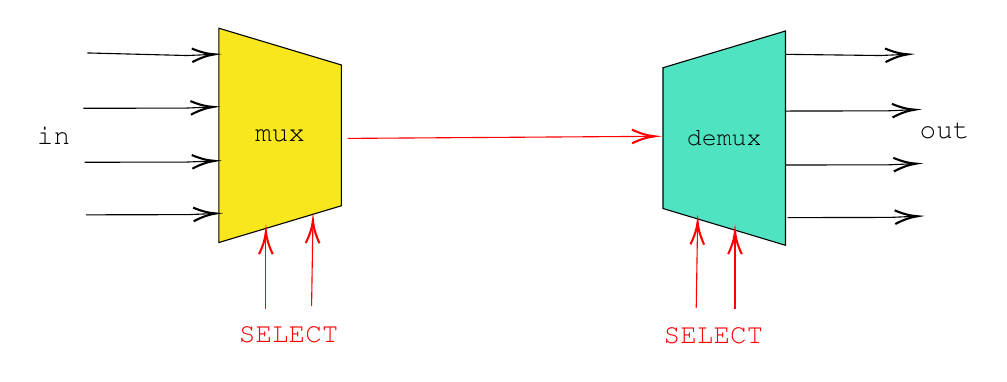
\begin{tikzpicture}[x=0.75pt,y=0.75pt,yscale=-1,xscale=1]
%uncomment if require: \path (0,300); %set diagram left start at 0, and has height of 300

%Shape: Trapezoid [id:dp9676716720394224] 
\draw  [fill={rgb, 255:red, 248; green, 231; blue, 28 }  ,fill opacity=1 ] (127,83.42) -- (186,101.12) -- (186,168.97) -- (127,186.67) -- cycle ;
%Shape: Trapezoid [id:dp8112150659093363] 
\draw  [fill={rgb, 255:red, 80; green, 227; blue, 194 }  ,fill opacity=1 ] (400,188) -- (341,170.3) -- (341,102.45) -- (400,84.75) -- cycle ;
%Straight Lines [id:da17513161874771777] 
\draw [color={rgb, 255:red, 255; green, 0; blue, 0 }  ,draw opacity=1 ]   (189,136.5) -- (335,135.51) ;
\draw [shift={(337,135.5)}, rotate = 539.61] [color={rgb, 255:red, 255; green, 0; blue, 0 }  ,draw opacity=1 ][line width=0.75]    (10.93,-3.29) .. controls (6.95,-1.4) and (3.31,-0.3) .. (0,0) .. controls (3.31,0.3) and (6.95,1.4) .. (10.93,3.29)   ;
%Straight Lines [id:da7314260725072124] 
\draw    (63.67,95.33) -- (111.64,96.57) -- (123,96.08) ;
\draw [shift={(125,96)}, rotate = 537.5699999999999] [color={rgb, 255:red, 0; green, 0; blue, 0 }  ][line width=0.75]    (10.93,-3.29) .. controls (6.95,-1.4) and (3.31,-0.3) .. (0,0) .. controls (3.31,0.3) and (6.95,1.4) .. (10.93,3.29)   ;
%Straight Lines [id:da32898600894177765] 
\draw    (61.67,122) -- (110.98,121.9) -- (122.34,121.42) ;
\draw [shift={(124.33,121.33)}, rotate = 537.5699999999999] [color={rgb, 255:red, 0; green, 0; blue, 0 }  ][line width=0.75]    (10.93,-3.29) .. controls (6.95,-1.4) and (3.31,-0.3) .. (0,0) .. controls (3.31,0.3) and (6.95,1.4) .. (10.93,3.29)   ;
%Straight Lines [id:da7983247275507934] 
\draw    (62.33,148) -- (111.64,147.9) -- (123,147.42) ;
\draw [shift={(125,147.33)}, rotate = 537.5699999999999] [color={rgb, 255:red, 0; green, 0; blue, 0 }  ][line width=0.75]    (10.93,-3.29) .. controls (6.95,-1.4) and (3.31,-0.3) .. (0,0) .. controls (3.31,0.3) and (6.95,1.4) .. (10.93,3.29)   ;
%Straight Lines [id:da04807653219902874] 
\draw    (63,173.33) -- (112.31,173.23) -- (123.67,172.75) ;
\draw [shift={(125.67,172.67)}, rotate = 537.5699999999999] [color={rgb, 255:red, 0; green, 0; blue, 0 }  ][line width=0.75]    (10.93,-3.29) .. controls (6.95,-1.4) and (3.31,-0.3) .. (0,0) .. controls (3.31,0.3) and (6.95,1.4) .. (10.93,3.29)   ;
%Straight Lines [id:da5159526044803394] 
\draw    (400.33,96) -- (445.64,96.57) -- (457,96.08) ;
\draw [shift={(459,96)}, rotate = 537.5699999999999] [color={rgb, 255:red, 0; green, 0; blue, 0 }  ][line width=0.75]    (10.93,-3.29) .. controls (6.95,-1.4) and (3.31,-0.3) .. (0,0) .. controls (3.31,0.3) and (6.95,1.4) .. (10.93,3.29)   ;
%Straight Lines [id:da8929745222846369] 
\draw    (399.67,123.33) -- (448.98,123.23) -- (460.34,122.75) ;
\draw [shift={(462.33,122.67)}, rotate = 537.5699999999999] [color={rgb, 255:red, 0; green, 0; blue, 0 }  ][line width=0.75]    (10.93,-3.29) .. controls (6.95,-1.4) and (3.31,-0.3) .. (0,0) .. controls (3.31,0.3) and (6.95,1.4) .. (10.93,3.29)   ;
%Straight Lines [id:da5083766804065095] 
\draw    (400.33,149.33) -- (449.64,149.23) -- (461,148.75) ;
\draw [shift={(463,148.67)}, rotate = 537.5699999999999] [color={rgb, 255:red, 0; green, 0; blue, 0 }  ][line width=0.75]    (10.93,-3.29) .. controls (6.95,-1.4) and (3.31,-0.3) .. (0,0) .. controls (3.31,0.3) and (6.95,1.4) .. (10.93,3.29)   ;
%Straight Lines [id:da4565821283716822] 
\draw    (401,174.67) -- (450.31,174.57) -- (461.67,174.08) ;
\draw [shift={(463.67,174)}, rotate = 537.5699999999999] [color={rgb, 255:red, 0; green, 0; blue, 0 }  ][line width=0.75]    (10.93,-3.29) .. controls (6.95,-1.4) and (3.31,-0.3) .. (0,0) .. controls (3.31,0.3) and (6.95,1.4) .. (10.93,3.29)   ;
%Straight Lines [id:da9657285985744374] 
\draw [color={rgb, 255:red, 255; green, 0; blue, 0 }  ,draw opacity=1 ][fill={rgb, 255:red, 255; green, 0; blue, 0 }  ,fill opacity=1 ]   (149.67,218.67) -- (149.67,183.33) ;
\draw [shift={(149.67,181.33)}, rotate = 450] [color={rgb, 255:red, 255; green, 0; blue, 0 }  ,draw opacity=1 ][line width=0.75]    (10.93,-3.29) .. controls (6.95,-1.4) and (3.31,-0.3) .. (0,0) .. controls (3.31,0.3) and (6.95,1.4) .. (10.93,3.29)   ;
%Straight Lines [id:da15318619740493855] 
\draw [color={rgb, 255:red, 255; green, 0; blue, 0 }  ,draw opacity=1 ]   (171.67,217.33) -- (172.3,178) ;
\draw [shift={(172.33,176)}, rotate = 450.92] [color={rgb, 255:red, 255; green, 0; blue, 0 }  ,draw opacity=1 ][line width=0.75]    (10.93,-3.29) .. controls (6.95,-1.4) and (3.31,-0.3) .. (0,0) .. controls (3.31,0.3) and (6.95,1.4) .. (10.93,3.29)   ;
%Straight Lines [id:da870193447515214] 
\draw [color={rgb, 255:red, 255; green, 0; blue, 0 }  ,draw opacity=1 ]   (375.67,218.67) -- (375.67,183.33) ;
\draw [shift={(375.67,181.33)}, rotate = 450] [color={rgb, 255:red, 255; green, 0; blue, 0 }  ,draw opacity=1 ][line width=0.75]    (10.93,-3.29) .. controls (6.95,-1.4) and (3.31,-0.3) .. (0,0) .. controls (3.31,0.3) and (6.95,1.4) .. (10.93,3.29)   ;
%Straight Lines [id:da69110814819773] 
\draw [color={rgb, 255:red, 255; green, 0; blue, 0 }  ,draw opacity=1 ]   (357,218) -- (357.63,178.67) ;
\draw [shift={(357.67,176.67)}, rotate = 450.92] [color={rgb, 255:red, 255; green, 0; blue, 0 }  ,draw opacity=1 ][line width=0.75]    (10.93,-3.29) .. controls (6.95,-1.4) and (3.31,-0.3) .. (0,0) .. controls (3.31,0.3) and (6.95,1.4) .. (10.93,3.29)   ;

% Text Node
\draw (160.67,231) node  [color={rgb, 255:red, 255; green, 0; blue, 0 }  ,opacity=1 ] [align=left] {{\fontfamily{pcr}\selectfont SELECT}};
% Text Node
\draw (365.33,231.67) node  [color={rgb, 255:red, 255; green, 0; blue, 0 }  ,opacity=1 ] [align=left] {{\fontfamily{pcr}\selectfont SELECT}};
% Text Node
\draw (47.33,135) node   [align=left] {{\fontfamily{pcr}\selectfont in}};
% Text Node
\draw (476.67,133) node   [align=left] {{\fontfamily{pcr}\selectfont out}};
% Text Node
\draw (156.5,135.04) node   [align=left] {{\fontfamily{pcr}\selectfont mux}};
% Text Node
\draw (370.5,136.38) node   [align=left] {{\fontfamily{pcr}\selectfont {\small demux}}};


\end{tikzpicture}

    	\end{frame}
    	
    	\begin{frame}
    		\frametitle{What can we observe?}
    		\begin{itemize}
    			\item If we want to signify which of the four inputs are being transmitted across the \texttt{OUTPUT} channel, we can go ahead and represent which one it is by using binary
    			
    		\end{itemize}
    		
    		
    		

\tikzset{every picture/.style={line width=0.75pt}} %set default line width to 0.75pt        

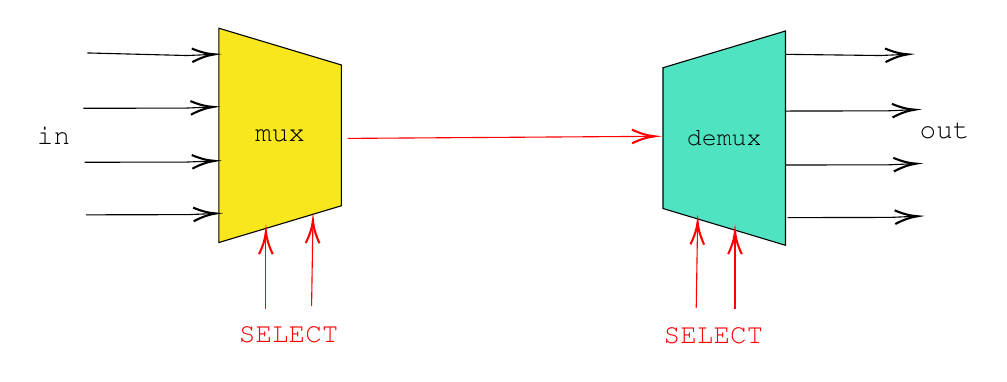
\begin{tikzpicture}[x=0.75pt,y=0.75pt,yscale=-1,xscale=1]
%uncomment if require: \path (0,300); %set diagram left start at 0, and has height of 300

%Shape: Trapezoid [id:dp9676716720394224] 
\draw  [fill={rgb, 255:red, 248; green, 231; blue, 28 }  ,fill opacity=1 ] (127,83.42) -- (186,101.12) -- (186,168.97) -- (127,186.67) -- cycle ;
%Shape: Trapezoid [id:dp8112150659093363] 
\draw  [fill={rgb, 255:red, 80; green, 227; blue, 194 }  ,fill opacity=1 ] (400,188) -- (341,170.3) -- (341,102.45) -- (400,84.75) -- cycle ;
%Straight Lines [id:da17513161874771777] 
\draw [color={rgb, 255:red, 255; green, 0; blue, 0 }  ,draw opacity=1 ]   (189,136.5) -- (335,135.51) ;
\draw [shift={(337,135.5)}, rotate = 539.61] [color={rgb, 255:red, 255; green, 0; blue, 0 }  ,draw opacity=1 ][line width=0.75]    (10.93,-3.29) .. controls (6.95,-1.4) and (3.31,-0.3) .. (0,0) .. controls (3.31,0.3) and (6.95,1.4) .. (10.93,3.29)   ;
%Straight Lines [id:da7314260725072124] 
\draw    (63.67,95.33) -- (111.64,96.57) -- (123,96.08) ;
\draw [shift={(125,96)}, rotate = 537.5699999999999] [color={rgb, 255:red, 0; green, 0; blue, 0 }  ][line width=0.75]    (10.93,-3.29) .. controls (6.95,-1.4) and (3.31,-0.3) .. (0,0) .. controls (3.31,0.3) and (6.95,1.4) .. (10.93,3.29)   ;
%Straight Lines [id:da32898600894177765] 
\draw    (61.67,122) -- (110.98,121.9) -- (122.34,121.42) ;
\draw [shift={(124.33,121.33)}, rotate = 537.5699999999999] [color={rgb, 255:red, 0; green, 0; blue, 0 }  ][line width=0.75]    (10.93,-3.29) .. controls (6.95,-1.4) and (3.31,-0.3) .. (0,0) .. controls (3.31,0.3) and (6.95,1.4) .. (10.93,3.29)   ;
%Straight Lines [id:da7983247275507934] 
\draw    (62.33,148) -- (111.64,147.9) -- (123,147.42) ;
\draw [shift={(125,147.33)}, rotate = 537.5699999999999] [color={rgb, 255:red, 0; green, 0; blue, 0 }  ][line width=0.75]    (10.93,-3.29) .. controls (6.95,-1.4) and (3.31,-0.3) .. (0,0) .. controls (3.31,0.3) and (6.95,1.4) .. (10.93,3.29)   ;
%Straight Lines [id:da04807653219902874] 
\draw    (63,173.33) -- (112.31,173.23) -- (123.67,172.75) ;
\draw [shift={(125.67,172.67)}, rotate = 537.5699999999999] [color={rgb, 255:red, 0; green, 0; blue, 0 }  ][line width=0.75]    (10.93,-3.29) .. controls (6.95,-1.4) and (3.31,-0.3) .. (0,0) .. controls (3.31,0.3) and (6.95,1.4) .. (10.93,3.29)   ;
%Straight Lines [id:da5159526044803394] 
\draw    (400.33,96) -- (445.64,96.57) -- (457,96.08) ;
\draw [shift={(459,96)}, rotate = 537.5699999999999] [color={rgb, 255:red, 0; green, 0; blue, 0 }  ][line width=0.75]    (10.93,-3.29) .. controls (6.95,-1.4) and (3.31,-0.3) .. (0,0) .. controls (3.31,0.3) and (6.95,1.4) .. (10.93,3.29)   ;
%Straight Lines [id:da8929745222846369] 
\draw    (399.67,123.33) -- (448.98,123.23) -- (460.34,122.75) ;
\draw [shift={(462.33,122.67)}, rotate = 537.5699999999999] [color={rgb, 255:red, 0; green, 0; blue, 0 }  ][line width=0.75]    (10.93,-3.29) .. controls (6.95,-1.4) and (3.31,-0.3) .. (0,0) .. controls (3.31,0.3) and (6.95,1.4) .. (10.93,3.29)   ;
%Straight Lines [id:da5083766804065095] 
\draw    (400.33,149.33) -- (449.64,149.23) -- (461,148.75) ;
\draw [shift={(463,148.67)}, rotate = 537.5699999999999] [color={rgb, 255:red, 0; green, 0; blue, 0 }  ][line width=0.75]    (10.93,-3.29) .. controls (6.95,-1.4) and (3.31,-0.3) .. (0,0) .. controls (3.31,0.3) and (6.95,1.4) .. (10.93,3.29)   ;
%Straight Lines [id:da4565821283716822] 
\draw    (401,174.67) -- (450.31,174.57) -- (461.67,174.08) ;
\draw [shift={(463.67,174)}, rotate = 537.5699999999999] [color={rgb, 255:red, 0; green, 0; blue, 0 }  ][line width=0.75]    (10.93,-3.29) .. controls (6.95,-1.4) and (3.31,-0.3) .. (0,0) .. controls (3.31,0.3) and (6.95,1.4) .. (10.93,3.29)   ;
%Straight Lines [id:da9657285985744374] 
\draw [color={rgb, 255:red, 255; green, 0; blue, 0 }  ,draw opacity=1 ][fill={rgb, 255:red, 255; green, 0; blue, 0 }  ,fill opacity=1 ]   (149.67,218.67) -- (149.67,183.33) ;
\draw [shift={(149.67,181.33)}, rotate = 450] [color={rgb, 255:red, 255; green, 0; blue, 0 }  ,draw opacity=1 ][line width=0.75]    (10.93,-3.29) .. controls (6.95,-1.4) and (3.31,-0.3) .. (0,0) .. controls (3.31,0.3) and (6.95,1.4) .. (10.93,3.29)   ;
%Straight Lines [id:da15318619740493855] 
\draw [color={rgb, 255:red, 255; green, 0; blue, 0 }  ,draw opacity=1 ]   (171.67,217.33) -- (172.3,178) ;
\draw [shift={(172.33,176)}, rotate = 450.92] [color={rgb, 255:red, 255; green, 0; blue, 0 }  ,draw opacity=1 ][line width=0.75]    (10.93,-3.29) .. controls (6.95,-1.4) and (3.31,-0.3) .. (0,0) .. controls (3.31,0.3) and (6.95,1.4) .. (10.93,3.29)   ;
%Straight Lines [id:da870193447515214] 
\draw [color={rgb, 255:red, 255; green, 0; blue, 0 }  ,draw opacity=1 ]   (375.67,218.67) -- (375.67,183.33) ;
\draw [shift={(375.67,181.33)}, rotate = 450] [color={rgb, 255:red, 255; green, 0; blue, 0 }  ,draw opacity=1 ][line width=0.75]    (10.93,-3.29) .. controls (6.95,-1.4) and (3.31,-0.3) .. (0,0) .. controls (3.31,0.3) and (6.95,1.4) .. (10.93,3.29)   ;
%Straight Lines [id:da69110814819773] 
\draw [color={rgb, 255:red, 255; green, 0; blue, 0 }  ,draw opacity=1 ]   (357,218) -- (357.63,178.67) ;
\draw [shift={(357.67,176.67)}, rotate = 450.92] [color={rgb, 255:red, 255; green, 0; blue, 0 }  ,draw opacity=1 ][line width=0.75]    (10.93,-3.29) .. controls (6.95,-1.4) and (3.31,-0.3) .. (0,0) .. controls (3.31,0.3) and (6.95,1.4) .. (10.93,3.29)   ;

% Text Node
\draw (160.67,231) node  [color={rgb, 255:red, 255; green, 0; blue, 0 }  ,opacity=1 ] [align=left] {{\fontfamily{pcr}\selectfont SELECT}};
% Text Node
\draw (365.33,231.67) node  [color={rgb, 255:red, 255; green, 0; blue, 0 }  ,opacity=1 ] [align=left] {{\fontfamily{pcr}\selectfont SELECT}};
% Text Node
\draw (47.33,135) node   [align=left] {{\fontfamily{pcr}\selectfont in}};
% Text Node
\draw (476.67,133) node   [align=left] {{\fontfamily{pcr}\selectfont out}};
% Text Node
\draw (156.5,135.04) node   [align=left] {{\fontfamily{pcr}\selectfont mux}};
% Text Node
\draw (370.5,136.38) node   [align=left] {{\fontfamily{pcr}\selectfont {\small demux}}};


\end{tikzpicture}

    	\end{frame}
    	
    	
    	\begin{frame}
			\frametitle{$4 \times 1$ Multiplexer \& Demultiplexer Example}
			

\tikzset{every picture/.style={line width=0.75pt}} %set default line width to 0.75pt        

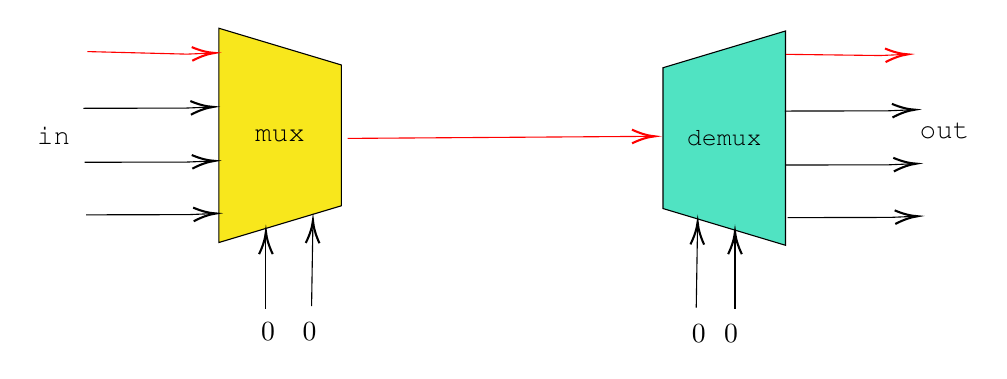
\begin{tikzpicture}[x=0.75pt,y=0.75pt,yscale=-1,xscale=1]
%uncomment if require: \path (0,300); %set diagram left start at 0, and has height of 300

%Shape: Trapezoid [id:dp9676716720394224] 
\draw  [fill={rgb, 255:red, 248; green, 231; blue, 28 }  ,fill opacity=1 ] (127,83.42) -- (186,101.12) -- (186,168.97) -- (127,186.67) -- cycle ;
%Shape: Trapezoid [id:dp8112150659093363] 
\draw  [fill={rgb, 255:red, 80; green, 227; blue, 194 }  ,fill opacity=1 ] (400,188) -- (341,170.3) -- (341,102.45) -- (400,84.75) -- cycle ;
%Straight Lines [id:da17513161874771777] 
\draw [color={rgb, 255:red, 255; green, 0; blue, 0 }  ,draw opacity=1 ]   (189,136.5) -- (335,135.51) ;
\draw [shift={(337,135.5)}, rotate = 539.61] [color={rgb, 255:red, 255; green, 0; blue, 0 }  ,draw opacity=1 ][line width=0.75]    (10.93,-3.29) .. controls (6.95,-1.4) and (3.31,-0.3) .. (0,0) .. controls (3.31,0.3) and (6.95,1.4) .. (10.93,3.29)   ;
%Straight Lines [id:da7314260725072124] 
\draw [color={rgb, 255:red, 255; green, 0; blue, 0 }  ,draw opacity=1 ]   (63.67,94.67) -- (111.64,95.9) -- (123,95.42) ;
\draw [shift={(125,95.33)}, rotate = 537.5699999999999] [color={rgb, 255:red, 255; green, 0; blue, 0 }  ,draw opacity=1 ][line width=0.75]    (10.93,-3.29) .. controls (6.95,-1.4) and (3.31,-0.3) .. (0,0) .. controls (3.31,0.3) and (6.95,1.4) .. (10.93,3.29)   ;
%Straight Lines [id:da32898600894177765] 
\draw    (61.67,122) -- (110.98,121.9) -- (122.34,121.42) ;
\draw [shift={(124.33,121.33)}, rotate = 537.5699999999999] [color={rgb, 255:red, 0; green, 0; blue, 0 }  ][line width=0.75]    (10.93,-3.29) .. controls (6.95,-1.4) and (3.31,-0.3) .. (0,0) .. controls (3.31,0.3) and (6.95,1.4) .. (10.93,3.29)   ;
%Straight Lines [id:da7983247275507934] 
\draw    (62.33,148) -- (111.64,147.9) -- (123,147.42) ;
\draw [shift={(125,147.33)}, rotate = 537.5699999999999] [color={rgb, 255:red, 0; green, 0; blue, 0 }  ][line width=0.75]    (10.93,-3.29) .. controls (6.95,-1.4) and (3.31,-0.3) .. (0,0) .. controls (3.31,0.3) and (6.95,1.4) .. (10.93,3.29)   ;
%Straight Lines [id:da04807653219902874] 
\draw    (63,173.33) -- (112.31,173.23) -- (123.67,172.75) ;
\draw [shift={(125.67,172.67)}, rotate = 537.5699999999999] [color={rgb, 255:red, 0; green, 0; blue, 0 }  ][line width=0.75]    (10.93,-3.29) .. controls (6.95,-1.4) and (3.31,-0.3) .. (0,0) .. controls (3.31,0.3) and (6.95,1.4) .. (10.93,3.29)   ;
%Straight Lines [id:da5159526044803394] 
\draw [color={rgb, 255:red, 255; green, 0; blue, 0 }  ,draw opacity=1 ]   (400.33,96) -- (445.64,96.57) -- (457,96.08) ;
\draw [shift={(459,96)}, rotate = 537.5699999999999] [color={rgb, 255:red, 255; green, 0; blue, 0 }  ,draw opacity=1 ][line width=0.75]    (10.93,-3.29) .. controls (6.95,-1.4) and (3.31,-0.3) .. (0,0) .. controls (3.31,0.3) and (6.95,1.4) .. (10.93,3.29)   ;
%Straight Lines [id:da8929745222846369] 
\draw    (399.67,123.33) -- (448.98,123.23) -- (460.34,122.75) ;
\draw [shift={(462.33,122.67)}, rotate = 537.5699999999999] [color={rgb, 255:red, 0; green, 0; blue, 0 }  ][line width=0.75]    (10.93,-3.29) .. controls (6.95,-1.4) and (3.31,-0.3) .. (0,0) .. controls (3.31,0.3) and (6.95,1.4) .. (10.93,3.29)   ;
%Straight Lines [id:da5083766804065095] 
\draw    (400.33,149.33) -- (449.64,149.23) -- (461,148.75) ;
\draw [shift={(463,148.67)}, rotate = 537.5699999999999] [color={rgb, 255:red, 0; green, 0; blue, 0 }  ][line width=0.75]    (10.93,-3.29) .. controls (6.95,-1.4) and (3.31,-0.3) .. (0,0) .. controls (3.31,0.3) and (6.95,1.4) .. (10.93,3.29)   ;
%Straight Lines [id:da4565821283716822] 
\draw    (401,174.67) -- (450.31,174.57) -- (461.67,174.08) ;
\draw [shift={(463.67,174)}, rotate = 537.5699999999999] [color={rgb, 255:red, 0; green, 0; blue, 0 }  ][line width=0.75]    (10.93,-3.29) .. controls (6.95,-1.4) and (3.31,-0.3) .. (0,0) .. controls (3.31,0.3) and (6.95,1.4) .. (10.93,3.29)   ;
%Straight Lines [id:da9657285985744374] 
\draw [color={rgb, 255:red, 0; green, 0; blue, 0 }  ,draw opacity=1 ][fill={rgb, 255:red, 255; green, 0; blue, 0 }  ,fill opacity=1 ]   (149.67,218.67) -- (149.67,183.33) ;
\draw [shift={(149.67,181.33)}, rotate = 450] [color={rgb, 255:red, 0; green, 0; blue, 0 }  ,draw opacity=1 ][line width=0.75]    (10.93,-3.29) .. controls (6.95,-1.4) and (3.31,-0.3) .. (0,0) .. controls (3.31,0.3) and (6.95,1.4) .. (10.93,3.29)   ;
%Straight Lines [id:da15318619740493855] 
\draw [color={rgb, 255:red, 0; green, 0; blue, 0 }  ,draw opacity=1 ]   (171.67,217.33) -- (172.3,178) ;
\draw [shift={(172.33,176)}, rotate = 450.92] [color={rgb, 255:red, 0; green, 0; blue, 0 }  ,draw opacity=1 ][line width=0.75]    (10.93,-3.29) .. controls (6.95,-1.4) and (3.31,-0.3) .. (0,0) .. controls (3.31,0.3) and (6.95,1.4) .. (10.93,3.29)   ;
%Straight Lines [id:da870193447515214] 
\draw [color={rgb, 255:red, 0; green, 0; blue, 0 }  ,draw opacity=1 ]   (375.67,218.67) -- (375.67,183.33) ;
\draw [shift={(375.67,181.33)}, rotate = 450] [color={rgb, 255:red, 0; green, 0; blue, 0 }  ,draw opacity=1 ][line width=0.75]    (10.93,-3.29) .. controls (6.95,-1.4) and (3.31,-0.3) .. (0,0) .. controls (3.31,0.3) and (6.95,1.4) .. (10.93,3.29)   ;
%Straight Lines [id:da69110814819773] 
\draw [color={rgb, 255:red, 0; green, 0; blue, 0 }  ,draw opacity=1 ]   (357,218) -- (357.63,178.67) ;
\draw [shift={(357.67,176.67)}, rotate = 450.92] [color={rgb, 255:red, 0; green, 0; blue, 0 }  ,draw opacity=1 ][line width=0.75]    (10.93,-3.29) .. controls (6.95,-1.4) and (3.31,-0.3) .. (0,0) .. controls (3.31,0.3) and (6.95,1.4) .. (10.93,3.29)   ;

% Text Node
\draw (160.67,229.67) node  [color={rgb, 255:red, 0; green, 0; blue, 0 }  ,opacity=1 ] [align=left] {0 \ \ 0};
% Text Node
\draw (366,230.33) node  [color={rgb, 255:red, 0; green, 0; blue, 0 }  ,opacity=1 ] [align=left] {0 \ 0};
% Text Node
\draw (47.33,135) node   [align=left] {{\fontfamily{pcr}\selectfont in}};
% Text Node
\draw (476.67,133) node   [align=left] {{\fontfamily{pcr}\selectfont out}};
% Text Node
\draw (156.5,135.04) node   [align=left] {{\fontfamily{pcr}\selectfont mux}};
% Text Node
\draw (370.5,136.38) node   [align=left] {{\fontfamily{pcr}\selectfont {\small demux}}};


\end{tikzpicture}
    		
    		
    	\end{frame}
    	
    	\begin{frame}
    		\frametitle{$4 \times 1$ Multiplexer \& Demultiplexer Example}
    		
    		

\tikzset{every picture/.style={line width=0.75pt}} %set default line width to 0.75pt        

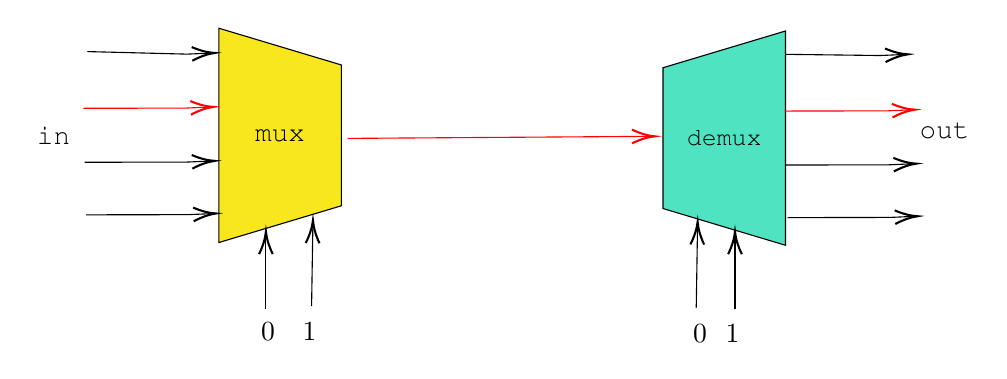
\begin{tikzpicture}[x=0.75pt,y=0.75pt,yscale=-1,xscale=1]
%uncomment if require: \path (0,300); %set diagram left start at 0, and has height of 300

%Shape: Trapezoid [id:dp9676716720394224] 
\draw  [fill={rgb, 255:red, 248; green, 231; blue, 28 }  ,fill opacity=1 ] (127,83.42) -- (186,101.12) -- (186,168.97) -- (127,186.67) -- cycle ;
%Shape: Trapezoid [id:dp8112150659093363] 
\draw  [fill={rgb, 255:red, 80; green, 227; blue, 194 }  ,fill opacity=1 ] (400,188) -- (341,170.3) -- (341,102.45) -- (400,84.75) -- cycle ;
%Straight Lines [id:da17513161874771777] 
\draw [color={rgb, 255:red, 255; green, 0; blue, 0 }  ,draw opacity=1 ]   (189,136.5) -- (335,135.51) ;
\draw [shift={(337,135.5)}, rotate = 539.61] [color={rgb, 255:red, 255; green, 0; blue, 0 }  ,draw opacity=1 ][line width=0.75]    (10.93,-3.29) .. controls (6.95,-1.4) and (3.31,-0.3) .. (0,0) .. controls (3.31,0.3) and (6.95,1.4) .. (10.93,3.29)   ;
%Straight Lines [id:da7314260725072124] 
\draw [color={rgb, 255:red, 0; green, 0; blue, 0 }  ,draw opacity=1 ]   (63.67,94.67) -- (111.64,95.9) -- (123,95.42) ;
\draw [shift={(125,95.33)}, rotate = 537.5699999999999] [color={rgb, 255:red, 0; green, 0; blue, 0 }  ,draw opacity=1 ][line width=0.75]    (10.93,-3.29) .. controls (6.95,-1.4) and (3.31,-0.3) .. (0,0) .. controls (3.31,0.3) and (6.95,1.4) .. (10.93,3.29)   ;
%Straight Lines [id:da32898600894177765] 
\draw [color={rgb, 255:red, 255; green, 0; blue, 0 }  ,draw opacity=1 ]   (61.67,122) -- (110.98,121.9) -- (122.34,121.42) ;
\draw [shift={(124.33,121.33)}, rotate = 537.5699999999999] [color={rgb, 255:red, 255; green, 0; blue, 0 }  ,draw opacity=1 ][line width=0.75]    (10.93,-3.29) .. controls (6.95,-1.4) and (3.31,-0.3) .. (0,0) .. controls (3.31,0.3) and (6.95,1.4) .. (10.93,3.29)   ;
%Straight Lines [id:da7983247275507934] 
\draw    (62.33,148) -- (111.64,147.9) -- (123,147.42) ;
\draw [shift={(125,147.33)}, rotate = 537.5699999999999] [color={rgb, 255:red, 0; green, 0; blue, 0 }  ][line width=0.75]    (10.93,-3.29) .. controls (6.95,-1.4) and (3.31,-0.3) .. (0,0) .. controls (3.31,0.3) and (6.95,1.4) .. (10.93,3.29)   ;
%Straight Lines [id:da04807653219902874] 
\draw    (63,173.33) -- (112.31,173.23) -- (123.67,172.75) ;
\draw [shift={(125.67,172.67)}, rotate = 537.5699999999999] [color={rgb, 255:red, 0; green, 0; blue, 0 }  ][line width=0.75]    (10.93,-3.29) .. controls (6.95,-1.4) and (3.31,-0.3) .. (0,0) .. controls (3.31,0.3) and (6.95,1.4) .. (10.93,3.29)   ;
%Straight Lines [id:da5159526044803394] 
\draw [color={rgb, 255:red, 0; green, 0; blue, 0 }  ,draw opacity=1 ]   (400.33,96) -- (445.64,96.57) -- (457,96.08) ;
\draw [shift={(459,96)}, rotate = 537.5699999999999] [color={rgb, 255:red, 0; green, 0; blue, 0 }  ,draw opacity=1 ][line width=0.75]    (10.93,-3.29) .. controls (6.95,-1.4) and (3.31,-0.3) .. (0,0) .. controls (3.31,0.3) and (6.95,1.4) .. (10.93,3.29)   ;
%Straight Lines [id:da8929745222846369] 
\draw [color={rgb, 255:red, 255; green, 0; blue, 0 }  ,draw opacity=1 ]   (399.67,123.33) -- (448.98,123.23) -- (460.34,122.75) ;
\draw [shift={(462.33,122.67)}, rotate = 537.5699999999999] [color={rgb, 255:red, 255; green, 0; blue, 0 }  ,draw opacity=1 ][line width=0.75]    (10.93,-3.29) .. controls (6.95,-1.4) and (3.31,-0.3) .. (0,0) .. controls (3.31,0.3) and (6.95,1.4) .. (10.93,3.29)   ;
%Straight Lines [id:da5083766804065095] 
\draw    (400.33,149.33) -- (449.64,149.23) -- (461,148.75) ;
\draw [shift={(463,148.67)}, rotate = 537.5699999999999] [color={rgb, 255:red, 0; green, 0; blue, 0 }  ][line width=0.75]    (10.93,-3.29) .. controls (6.95,-1.4) and (3.31,-0.3) .. (0,0) .. controls (3.31,0.3) and (6.95,1.4) .. (10.93,3.29)   ;
%Straight Lines [id:da4565821283716822] 
\draw    (401,174.67) -- (450.31,174.57) -- (461.67,174.08) ;
\draw [shift={(463.67,174)}, rotate = 537.5699999999999] [color={rgb, 255:red, 0; green, 0; blue, 0 }  ][line width=0.75]    (10.93,-3.29) .. controls (6.95,-1.4) and (3.31,-0.3) .. (0,0) .. controls (3.31,0.3) and (6.95,1.4) .. (10.93,3.29)   ;
%Straight Lines [id:da9657285985744374] 
\draw [color={rgb, 255:red, 0; green, 0; blue, 0 }  ,draw opacity=1 ][fill={rgb, 255:red, 255; green, 0; blue, 0 }  ,fill opacity=1 ]   (149.67,218.67) -- (149.67,183.33) ;
\draw [shift={(149.67,181.33)}, rotate = 450] [color={rgb, 255:red, 0; green, 0; blue, 0 }  ,draw opacity=1 ][line width=0.75]    (10.93,-3.29) .. controls (6.95,-1.4) and (3.31,-0.3) .. (0,0) .. controls (3.31,0.3) and (6.95,1.4) .. (10.93,3.29)   ;
%Straight Lines [id:da15318619740493855] 
\draw [color={rgb, 255:red, 0; green, 0; blue, 0 }  ,draw opacity=1 ]   (171.67,217.33) -- (172.3,178) ;
\draw [shift={(172.33,176)}, rotate = 450.92] [color={rgb, 255:red, 0; green, 0; blue, 0 }  ,draw opacity=1 ][line width=0.75]    (10.93,-3.29) .. controls (6.95,-1.4) and (3.31,-0.3) .. (0,0) .. controls (3.31,0.3) and (6.95,1.4) .. (10.93,3.29)   ;
%Straight Lines [id:da870193447515214] 
\draw [color={rgb, 255:red, 0; green, 0; blue, 0 }  ,draw opacity=1 ]   (375.67,218.67) -- (375.67,183.33) ;
\draw [shift={(375.67,181.33)}, rotate = 450] [color={rgb, 255:red, 0; green, 0; blue, 0 }  ,draw opacity=1 ][line width=0.75]    (10.93,-3.29) .. controls (6.95,-1.4) and (3.31,-0.3) .. (0,0) .. controls (3.31,0.3) and (6.95,1.4) .. (10.93,3.29)   ;
%Straight Lines [id:da69110814819773] 
\draw [color={rgb, 255:red, 0; green, 0; blue, 0 }  ,draw opacity=1 ]   (357,218) -- (357.63,178.67) ;
\draw [shift={(357.67,176.67)}, rotate = 450.92] [color={rgb, 255:red, 0; green, 0; blue, 0 }  ,draw opacity=1 ][line width=0.75]    (10.93,-3.29) .. controls (6.95,-1.4) and (3.31,-0.3) .. (0,0) .. controls (3.31,0.3) and (6.95,1.4) .. (10.93,3.29)   ;

% Text Node
\draw (160.67,229.67) node  [color={rgb, 255:red, 0; green, 0; blue, 0 }  ,opacity=1 ] [align=left] {0 \ \ 1};
% Text Node
\draw (366.67,230.33) node  [color={rgb, 255:red, 0; green, 0; blue, 0 }  ,opacity=1 ] [align=left] {0 \ 1};
% Text Node
\draw (47.33,135) node   [align=left] {{\fontfamily{pcr}\selectfont in}};
% Text Node
\draw (476.67,133) node   [align=left] {{\fontfamily{pcr}\selectfont out}};
% Text Node
\draw (156.5,135.04) node   [align=left] {{\fontfamily{pcr}\selectfont mux}};
% Text Node
\draw (370.5,136.38) node   [align=left] {{\fontfamily{pcr}\selectfont {\small demux}}};


\end{tikzpicture}

    	\end{frame}
    	
    	
    	\begin{frame}
    		\frametitle{$4 \times 1$ Multiplexer \& Demultiplexer Example}
    		
    		

\tikzset{every picture/.style={line width=0.75pt}} %set default line width to 0.75pt        

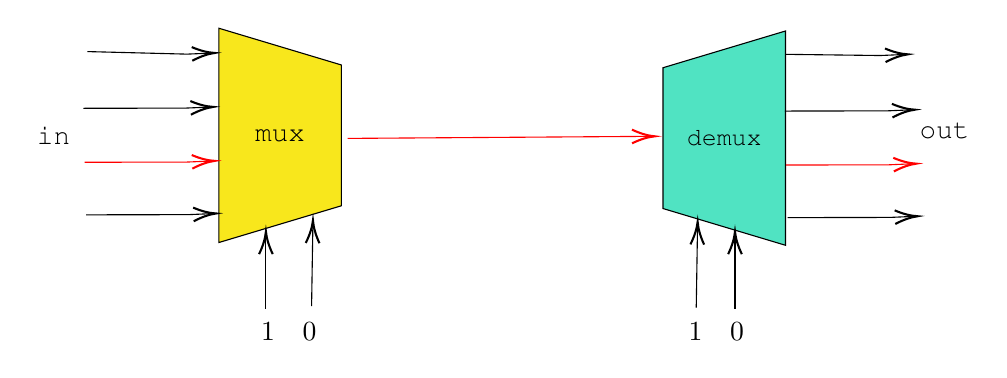
\begin{tikzpicture}[x=0.75pt,y=0.75pt,yscale=-1,xscale=1]
%uncomment if require: \path (0,300); %set diagram left start at 0, and has height of 300

%Shape: Trapezoid [id:dp9676716720394224] 
\draw  [fill={rgb, 255:red, 248; green, 231; blue, 28 }  ,fill opacity=1 ] (127,83.42) -- (186,101.12) -- (186,168.97) -- (127,186.67) -- cycle ;
%Shape: Trapezoid [id:dp8112150659093363] 
\draw  [fill={rgb, 255:red, 80; green, 227; blue, 194 }  ,fill opacity=1 ] (400,188) -- (341,170.3) -- (341,102.45) -- (400,84.75) -- cycle ;
%Straight Lines [id:da17513161874771777] 
\draw [color={rgb, 255:red, 255; green, 0; blue, 0 }  ,draw opacity=1 ]   (189,136.5) -- (335,135.51) ;
\draw [shift={(337,135.5)}, rotate = 539.61] [color={rgb, 255:red, 255; green, 0; blue, 0 }  ,draw opacity=1 ][line width=0.75]    (10.93,-3.29) .. controls (6.95,-1.4) and (3.31,-0.3) .. (0,0) .. controls (3.31,0.3) and (6.95,1.4) .. (10.93,3.29)   ;
%Straight Lines [id:da7314260725072124] 
\draw [color={rgb, 255:red, 0; green, 0; blue, 0 }  ,draw opacity=1 ]   (63.67,94.67) -- (111.64,95.9) -- (123,95.42) ;
\draw [shift={(125,95.33)}, rotate = 537.5699999999999] [color={rgb, 255:red, 0; green, 0; blue, 0 }  ,draw opacity=1 ][line width=0.75]    (10.93,-3.29) .. controls (6.95,-1.4) and (3.31,-0.3) .. (0,0) .. controls (3.31,0.3) and (6.95,1.4) .. (10.93,3.29)   ;
%Straight Lines [id:da32898600894177765] 
\draw [color={rgb, 255:red, 0; green, 0; blue, 0 }  ,draw opacity=1 ]   (61.67,122) -- (110.98,121.9) -- (122.34,121.42) ;
\draw [shift={(124.33,121.33)}, rotate = 537.5699999999999] [color={rgb, 255:red, 0; green, 0; blue, 0 }  ,draw opacity=1 ][line width=0.75]    (10.93,-3.29) .. controls (6.95,-1.4) and (3.31,-0.3) .. (0,0) .. controls (3.31,0.3) and (6.95,1.4) .. (10.93,3.29)   ;
%Straight Lines [id:da7983247275507934] 
\draw [color={rgb, 255:red, 255; green, 0; blue, 0 }  ,draw opacity=1 ]   (62.33,148) -- (111.64,147.9) -- (123,147.42) ;
\draw [shift={(125,147.33)}, rotate = 537.5699999999999] [color={rgb, 255:red, 255; green, 0; blue, 0 }  ,draw opacity=1 ][line width=0.75]    (10.93,-3.29) .. controls (6.95,-1.4) and (3.31,-0.3) .. (0,0) .. controls (3.31,0.3) and (6.95,1.4) .. (10.93,3.29)   ;
%Straight Lines [id:da04807653219902874] 
\draw    (63,173.33) -- (112.31,173.23) -- (123.67,172.75) ;
\draw [shift={(125.67,172.67)}, rotate = 537.5699999999999] [color={rgb, 255:red, 0; green, 0; blue, 0 }  ][line width=0.75]    (10.93,-3.29) .. controls (6.95,-1.4) and (3.31,-0.3) .. (0,0) .. controls (3.31,0.3) and (6.95,1.4) .. (10.93,3.29)   ;
%Straight Lines [id:da5159526044803394] 
\draw [color={rgb, 255:red, 0; green, 0; blue, 0 }  ,draw opacity=1 ]   (400.33,96) -- (445.64,96.57) -- (457,96.08) ;
\draw [shift={(459,96)}, rotate = 537.5699999999999] [color={rgb, 255:red, 0; green, 0; blue, 0 }  ,draw opacity=1 ][line width=0.75]    (10.93,-3.29) .. controls (6.95,-1.4) and (3.31,-0.3) .. (0,0) .. controls (3.31,0.3) and (6.95,1.4) .. (10.93,3.29)   ;
%Straight Lines [id:da8929745222846369] 
\draw [color={rgb, 255:red, 0; green, 0; blue, 0 }  ,draw opacity=1 ]   (399.67,123.33) -- (448.98,123.23) -- (460.34,122.75) ;
\draw [shift={(462.33,122.67)}, rotate = 537.5699999999999] [color={rgb, 255:red, 0; green, 0; blue, 0 }  ,draw opacity=1 ][line width=0.75]    (10.93,-3.29) .. controls (6.95,-1.4) and (3.31,-0.3) .. (0,0) .. controls (3.31,0.3) and (6.95,1.4) .. (10.93,3.29)   ;
%Straight Lines [id:da5083766804065095] 
\draw [color={rgb, 255:red, 255; green, 0; blue, 0 }  ,draw opacity=1 ]   (400.33,149.33) -- (449.64,149.23) -- (461,148.75) ;
\draw [shift={(463,148.67)}, rotate = 537.5699999999999] [color={rgb, 255:red, 255; green, 0; blue, 0 }  ,draw opacity=1 ][line width=0.75]    (10.93,-3.29) .. controls (6.95,-1.4) and (3.31,-0.3) .. (0,0) .. controls (3.31,0.3) and (6.95,1.4) .. (10.93,3.29)   ;
%Straight Lines [id:da4565821283716822] 
\draw    (401,174.67) -- (450.31,174.57) -- (461.67,174.08) ;
\draw [shift={(463.67,174)}, rotate = 537.5699999999999] [color={rgb, 255:red, 0; green, 0; blue, 0 }  ][line width=0.75]    (10.93,-3.29) .. controls (6.95,-1.4) and (3.31,-0.3) .. (0,0) .. controls (3.31,0.3) and (6.95,1.4) .. (10.93,3.29)   ;
%Straight Lines [id:da9657285985744374] 
\draw [color={rgb, 255:red, 0; green, 0; blue, 0 }  ,draw opacity=1 ][fill={rgb, 255:red, 255; green, 0; blue, 0 }  ,fill opacity=1 ]   (149.67,218.67) -- (149.67,183.33) ;
\draw [shift={(149.67,181.33)}, rotate = 450] [color={rgb, 255:red, 0; green, 0; blue, 0 }  ,draw opacity=1 ][line width=0.75]    (10.93,-3.29) .. controls (6.95,-1.4) and (3.31,-0.3) .. (0,0) .. controls (3.31,0.3) and (6.95,1.4) .. (10.93,3.29)   ;
%Straight Lines [id:da15318619740493855] 
\draw [color={rgb, 255:red, 0; green, 0; blue, 0 }  ,draw opacity=1 ]   (171.67,217.33) -- (172.3,178) ;
\draw [shift={(172.33,176)}, rotate = 450.92] [color={rgb, 255:red, 0; green, 0; blue, 0 }  ,draw opacity=1 ][line width=0.75]    (10.93,-3.29) .. controls (6.95,-1.4) and (3.31,-0.3) .. (0,0) .. controls (3.31,0.3) and (6.95,1.4) .. (10.93,3.29)   ;
%Straight Lines [id:da870193447515214] 
\draw [color={rgb, 255:red, 0; green, 0; blue, 0 }  ,draw opacity=1 ]   (375.67,218.67) -- (375.67,183.33) ;
\draw [shift={(375.67,181.33)}, rotate = 450] [color={rgb, 255:red, 0; green, 0; blue, 0 }  ,draw opacity=1 ][line width=0.75]    (10.93,-3.29) .. controls (6.95,-1.4) and (3.31,-0.3) .. (0,0) .. controls (3.31,0.3) and (6.95,1.4) .. (10.93,3.29)   ;
%Straight Lines [id:da69110814819773] 
\draw [color={rgb, 255:red, 0; green, 0; blue, 0 }  ,draw opacity=1 ]   (357,218) -- (357.63,178.67) ;
\draw [shift={(357.67,176.67)}, rotate = 450.92] [color={rgb, 255:red, 0; green, 0; blue, 0 }  ,draw opacity=1 ][line width=0.75]    (10.93,-3.29) .. controls (6.95,-1.4) and (3.31,-0.3) .. (0,0) .. controls (3.31,0.3) and (6.95,1.4) .. (10.93,3.29)   ;

% Text Node
\draw (160.67,229.67) node  [color={rgb, 255:red, 0; green, 0; blue, 0 }  ,opacity=1 ] [align=left] {1 \ \ 0};
% Text Node
\draw (366.67,229.67) node  [color={rgb, 255:red, 0; green, 0; blue, 0 }  ,opacity=1 ] [align=left] {1 \ \ 0};
% Text Node
\draw (47.33,135) node   [align=left] {{\fontfamily{pcr}\selectfont in}};
% Text Node
\draw (476.67,133) node   [align=left] {{\fontfamily{pcr}\selectfont out}};
% Text Node
\draw (156.5,135.04) node   [align=left] {{\fontfamily{pcr}\selectfont mux}};
% Text Node
\draw (370.5,136.38) node   [align=left] {{\fontfamily{pcr}\selectfont {\small demux}}};


\end{tikzpicture}

    	\end{frame}
    	
    	\begin{frame}
    		\frametitle{$4 \times 1$ Multiplexer \& Demultiplexer Example}
    		
    		

\tikzset{every picture/.style={line width=0.75pt}} %set default line width to 0.75pt        

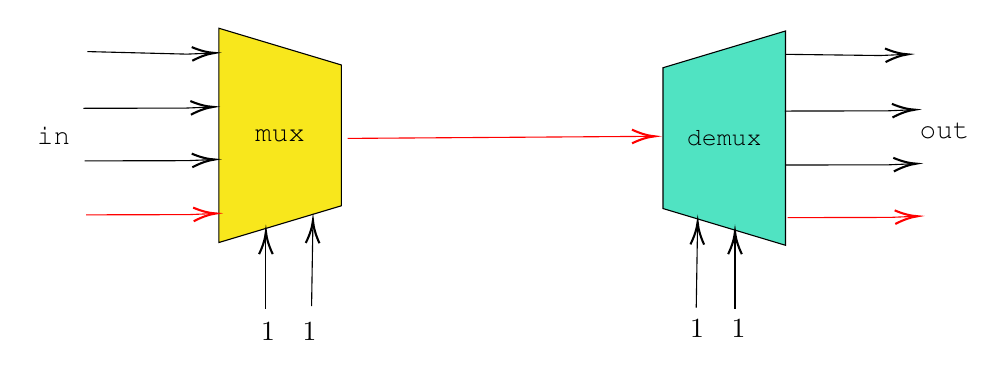
\begin{tikzpicture}[x=0.75pt,y=0.75pt,yscale=-1,xscale=1]
%uncomment if require: \path (0,300); %set diagram left start at 0, and has height of 300

%Shape: Trapezoid [id:dp9676716720394224] 
\draw  [fill={rgb, 255:red, 248; green, 231; blue, 28 }  ,fill opacity=1 ] (127,83.42) -- (186,101.12) -- (186,168.97) -- (127,186.67) -- cycle ;
%Shape: Trapezoid [id:dp8112150659093363] 
\draw  [fill={rgb, 255:red, 80; green, 227; blue, 194 }  ,fill opacity=1 ] (400,188) -- (341,170.3) -- (341,102.45) -- (400,84.75) -- cycle ;
%Straight Lines [id:da17513161874771777] 
\draw [color={rgb, 255:red, 255; green, 0; blue, 0 }  ,draw opacity=1 ]   (189,136.5) -- (335,135.51) ;
\draw [shift={(337,135.5)}, rotate = 539.61] [color={rgb, 255:red, 255; green, 0; blue, 0 }  ,draw opacity=1 ][line width=0.75]    (10.93,-3.29) .. controls (6.95,-1.4) and (3.31,-0.3) .. (0,0) .. controls (3.31,0.3) and (6.95,1.4) .. (10.93,3.29)   ;
%Straight Lines [id:da7314260725072124] 
\draw [color={rgb, 255:red, 0; green, 0; blue, 0 }  ,draw opacity=1 ]   (63.67,94.67) -- (111.64,95.9) -- (123,95.42) ;
\draw [shift={(125,95.33)}, rotate = 537.5699999999999] [color={rgb, 255:red, 0; green, 0; blue, 0 }  ,draw opacity=1 ][line width=0.75]    (10.93,-3.29) .. controls (6.95,-1.4) and (3.31,-0.3) .. (0,0) .. controls (3.31,0.3) and (6.95,1.4) .. (10.93,3.29)   ;
%Straight Lines [id:da32898600894177765] 
\draw [color={rgb, 255:red, 0; green, 0; blue, 0 }  ,draw opacity=1 ]   (61.67,122) -- (110.98,121.9) -- (122.34,121.42) ;
\draw [shift={(124.33,121.33)}, rotate = 537.5699999999999] [color={rgb, 255:red, 0; green, 0; blue, 0 }  ,draw opacity=1 ][line width=0.75]    (10.93,-3.29) .. controls (6.95,-1.4) and (3.31,-0.3) .. (0,0) .. controls (3.31,0.3) and (6.95,1.4) .. (10.93,3.29)   ;
%Straight Lines [id:da7983247275507934] 
\draw [color={rgb, 255:red, 0; green, 0; blue, 0 }  ,draw opacity=1 ]   (62.33,147.33) -- (111.64,147.23) -- (123,146.75) ;
\draw [shift={(125,146.67)}, rotate = 537.5699999999999] [color={rgb, 255:red, 0; green, 0; blue, 0 }  ,draw opacity=1 ][line width=0.75]    (10.93,-3.29) .. controls (6.95,-1.4) and (3.31,-0.3) .. (0,0) .. controls (3.31,0.3) and (6.95,1.4) .. (10.93,3.29)   ;
%Straight Lines [id:da04807653219902874] 
\draw [color={rgb, 255:red, 255; green, 0; blue, 0 }  ,draw opacity=1 ]   (63,173.33) -- (112.31,173.23) -- (123.67,172.75) ;
\draw [shift={(125.67,172.67)}, rotate = 537.5699999999999] [color={rgb, 255:red, 255; green, 0; blue, 0 }  ,draw opacity=1 ][line width=0.75]    (10.93,-3.29) .. controls (6.95,-1.4) and (3.31,-0.3) .. (0,0) .. controls (3.31,0.3) and (6.95,1.4) .. (10.93,3.29)   ;
%Straight Lines [id:da5159526044803394] 
\draw [color={rgb, 255:red, 0; green, 0; blue, 0 }  ,draw opacity=1 ]   (400.33,96) -- (445.64,96.57) -- (457,96.08) ;
\draw [shift={(459,96)}, rotate = 537.5699999999999] [color={rgb, 255:red, 0; green, 0; blue, 0 }  ,draw opacity=1 ][line width=0.75]    (10.93,-3.29) .. controls (6.95,-1.4) and (3.31,-0.3) .. (0,0) .. controls (3.31,0.3) and (6.95,1.4) .. (10.93,3.29)   ;
%Straight Lines [id:da8929745222846369] 
\draw [color={rgb, 255:red, 0; green, 0; blue, 0 }  ,draw opacity=1 ]   (399.67,123.33) -- (448.98,123.23) -- (460.34,122.75) ;
\draw [shift={(462.33,122.67)}, rotate = 537.5699999999999] [color={rgb, 255:red, 0; green, 0; blue, 0 }  ,draw opacity=1 ][line width=0.75]    (10.93,-3.29) .. controls (6.95,-1.4) and (3.31,-0.3) .. (0,0) .. controls (3.31,0.3) and (6.95,1.4) .. (10.93,3.29)   ;
%Straight Lines [id:da5083766804065095] 
\draw [color={rgb, 255:red, 0; green, 0; blue, 0 }  ,draw opacity=1 ]   (400.33,149.33) -- (449.64,149.23) -- (461,148.75) ;
\draw [shift={(463,148.67)}, rotate = 537.5699999999999] [color={rgb, 255:red, 0; green, 0; blue, 0 }  ,draw opacity=1 ][line width=0.75]    (10.93,-3.29) .. controls (6.95,-1.4) and (3.31,-0.3) .. (0,0) .. controls (3.31,0.3) and (6.95,1.4) .. (10.93,3.29)   ;
%Straight Lines [id:da4565821283716822] 
\draw [color={rgb, 255:red, 255; green, 0; blue, 0 }  ,draw opacity=1 ]   (401,174.67) -- (450.31,174.57) -- (461.67,174.08) ;
\draw [shift={(463.67,174)}, rotate = 537.5699999999999] [color={rgb, 255:red, 255; green, 0; blue, 0 }  ,draw opacity=1 ][line width=0.75]    (10.93,-3.29) .. controls (6.95,-1.4) and (3.31,-0.3) .. (0,0) .. controls (3.31,0.3) and (6.95,1.4) .. (10.93,3.29)   ;
%Straight Lines [id:da9657285985744374] 
\draw [color={rgb, 255:red, 0; green, 0; blue, 0 }  ,draw opacity=1 ][fill={rgb, 255:red, 255; green, 0; blue, 0 }  ,fill opacity=1 ]   (149.67,218.67) -- (149.67,183.33) ;
\draw [shift={(149.67,181.33)}, rotate = 450] [color={rgb, 255:red, 0; green, 0; blue, 0 }  ,draw opacity=1 ][line width=0.75]    (10.93,-3.29) .. controls (6.95,-1.4) and (3.31,-0.3) .. (0,0) .. controls (3.31,0.3) and (6.95,1.4) .. (10.93,3.29)   ;
%Straight Lines [id:da15318619740493855] 
\draw [color={rgb, 255:red, 0; green, 0; blue, 0 }  ,draw opacity=1 ]   (171.67,217.33) -- (172.3,178) ;
\draw [shift={(172.33,176)}, rotate = 450.92] [color={rgb, 255:red, 0; green, 0; blue, 0 }  ,draw opacity=1 ][line width=0.75]    (10.93,-3.29) .. controls (6.95,-1.4) and (3.31,-0.3) .. (0,0) .. controls (3.31,0.3) and (6.95,1.4) .. (10.93,3.29)   ;
%Straight Lines [id:da870193447515214] 
\draw [color={rgb, 255:red, 0; green, 0; blue, 0 }  ,draw opacity=1 ]   (375.67,218.67) -- (375.67,183.33) ;
\draw [shift={(375.67,181.33)}, rotate = 450] [color={rgb, 255:red, 0; green, 0; blue, 0 }  ,draw opacity=1 ][line width=0.75]    (10.93,-3.29) .. controls (6.95,-1.4) and (3.31,-0.3) .. (0,0) .. controls (3.31,0.3) and (6.95,1.4) .. (10.93,3.29)   ;
%Straight Lines [id:da69110814819773] 
\draw [color={rgb, 255:red, 0; green, 0; blue, 0 }  ,draw opacity=1 ]   (357,218) -- (357.63,178.67) ;
\draw [shift={(357.67,176.67)}, rotate = 450.92] [color={rgb, 255:red, 0; green, 0; blue, 0 }  ,draw opacity=1 ][line width=0.75]    (10.93,-3.29) .. controls (6.95,-1.4) and (3.31,-0.3) .. (0,0) .. controls (3.31,0.3) and (6.95,1.4) .. (10.93,3.29)   ;

% Text Node
\draw (160.67,229.67) node  [color={rgb, 255:red, 0; green, 0; blue, 0 }  ,opacity=1 ] [align=left] {1 \ \ 1};
% Text Node
\draw (367.33,228.33) node  [color={rgb, 255:red, 0; green, 0; blue, 0 }  ,opacity=1 ] [align=left] {1 \ \ 1};
% Text Node
\draw (47.33,135) node   [align=left] {{\fontfamily{pcr}\selectfont in}};
% Text Node
\draw (476.67,133) node   [align=left] {{\fontfamily{pcr}\selectfont out}};
% Text Node
\draw (156.5,135.04) node   [align=left] {{\fontfamily{pcr}\selectfont mux}};
% Text Node
\draw (370.5,136.38) node   [align=left] {{\fontfamily{pcr}\selectfont {\small demux}}};


\end{tikzpicture}

    	\end{frame}
    	
    	
    	\begin{frame}
			\frametitle{Immediate Observations}
			\begin{itemize}
				\item We need less wires to carry signals across long distances (this is good!)
				\item We can only carry one signal across this channel at once (this may be bad!)
				\item In summary- it's all about tradeoffs
			\end{itemize}			    		
    		
    	\end{frame}
    	
    	
    	\subsection{Muxes and Demuxes In-Depth}
    	
    	
    	\begin{frame}
                \vfill
                \centering
                \begin{beamercolorbox}[sep=8pt,center,shadow=true,rounded=true]{title}
                    \usebeamerfont{title}Muxes \& Demuxes In-depth\par%
                \end{beamercolorbox}
                \vfill
             \end{frame}
             
             \begin{frame}
             	\frametitle{Multiplexer}
             	
             	\begin{itemize}
             		\item Now that we understand multiplexers conceptually, can you think of how you'd build it with the logic gates we've learned? 
             	\end{itemize}
             	
             	\centering
             	

\tikzset{every picture/.style={line width=0.75pt}} %set default line width to 0.75pt        

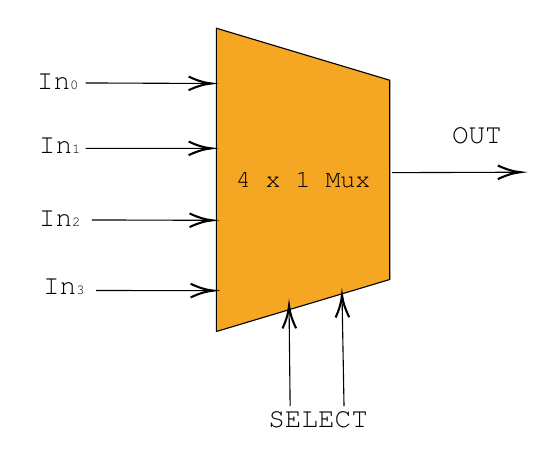
\begin{tikzpicture}[x=0.75pt,y=0.75pt,yscale=-1,xscale=1]
%uncomment if require: \path (0,300); %set diagram left start at 0, and has height of 300

%Shape: Trapezoid [id:dp8819284031411343] 
\draw  [fill={rgb, 255:red, 245; green, 166; blue, 35 }  ,fill opacity=1 ] (234,63.88) -- (317.5,88.93) -- (317.5,184.95) -- (234,210) -- cycle ;
%Straight Lines [id:da018103449442484876] 
\draw    (171,90.25) -- (229.54,90.49) ;
\draw [shift={(231.54,90.5)}, rotate = 180.24] [color={rgb, 255:red, 0; green, 0; blue, 0 }  ][line width=0.75]    (10.93,-3.29) .. controls (6.95,-1.4) and (3.31,-0.3) .. (0,0) .. controls (3.31,0.3) and (6.95,1.4) .. (10.93,3.29)   ;
%Straight Lines [id:da27398747593297434] 
\draw    (171,121.75) -- (229.54,121.76) ;
\draw [shift={(231.54,121.76)}, rotate = 180.01] [color={rgb, 255:red, 0; green, 0; blue, 0 }  ][line width=0.75]    (10.93,-3.29) .. controls (6.95,-1.4) and (3.31,-0.3) .. (0,0) .. controls (3.31,0.3) and (6.95,1.4) .. (10.93,3.29)   ;
%Straight Lines [id:da45011870969451995] 
\draw    (174,156.25) -- (230,156.42) ;
\draw [shift={(232,156.43)}, rotate = 180.18] [color={rgb, 255:red, 0; green, 0; blue, 0 }  ][line width=0.75]    (10.93,-3.29) .. controls (6.95,-1.4) and (3.31,-0.3) .. (0,0) .. controls (3.31,0.3) and (6.95,1.4) .. (10.93,3.29)   ;
%Straight Lines [id:da3811016173438192] 
\draw    (176,190.25) -- (230.5,190.3) ;
\draw [shift={(232.5,190.3)}, rotate = 180.05] [color={rgb, 255:red, 0; green, 0; blue, 0 }  ][line width=0.75]    (10.93,-3.29) .. controls (6.95,-1.4) and (3.31,-0.3) .. (0,0) .. controls (3.31,0.3) and (6.95,1.4) .. (10.93,3.29)   ;
%Straight Lines [id:da3695279660393864] 
\draw    (318.5,133.46) -- (378.5,133.26) ;
\draw [shift={(380.5,133.25)}, rotate = 539.8] [color={rgb, 255:red, 0; green, 0; blue, 0 }  ][line width=0.75]    (10.93,-3.29) .. controls (6.95,-1.4) and (3.31,-0.3) .. (0,0) .. controls (3.31,0.3) and (6.95,1.4) .. (10.93,3.29)   ;
%Straight Lines [id:da8955779809256085] 
\draw    (269.5,246) -- (269.01,199.56) ;
\draw [shift={(268.99,197.56)}, rotate = 449.4] [color={rgb, 255:red, 0; green, 0; blue, 0 }  ][line width=0.75]    (10.93,-3.29) .. controls (6.95,-1.4) and (3.31,-0.3) .. (0,0) .. controls (3.31,0.3) and (6.95,1.4) .. (10.93,3.29)   ;
%Straight Lines [id:da2688029751798525] 
\draw    (295.47,245.93) -- (294.54,194.25) ;
\draw [shift={(294.5,192.25)}, rotate = 448.97] [color={rgb, 255:red, 0; green, 0; blue, 0 }  ][line width=0.75]    (10.93,-3.29) .. controls (6.95,-1.4) and (3.31,-0.3) .. (0,0) .. controls (3.31,0.3) and (6.95,1.4) .. (10.93,3.29)   ;

% Text Node
\draw (157.5,89.5) node   [align=left] {{\fontfamily{pcr}\selectfont In{\tiny 0}}};
% Text Node
\draw (158.5,120.5) node   [align=left] {{\fontfamily{pcr}\selectfont In{\tiny 1}}};
% Text Node
\draw (158.5,155.5) node   [align=left] {{\fontfamily{pcr}\selectfont In{\tiny 2}}};
% Text Node
\draw (160.5,188.5) node   [align=left] {{\fontfamily{pcr}\selectfont In{\tiny 3}}};
% Text Node
\draw (283,252.5) node   [align=left] {{\fontfamily{pcr}\selectfont SELECT}};
% Text Node
\draw (359.5,115.5) node   [align=left] {{\fontfamily{pcr}\selectfont OUT}};
% Text Node
\draw (275.75,136.94) node   [align=left] {{\fontfamily{pcr}\selectfont {\small 4 x 1 Mux}}};


\end{tikzpicture}

             \end{frame}
             
             \begin{frame}
             	\frametitle{Multiplexer}
             	\begin{itemize}
             		\item Here's the actual logical circuit
             	\end{itemize}
             	\centering
             	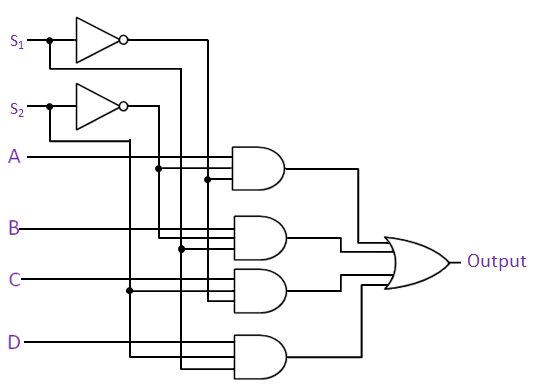
\includegraphics[width=0.7\textwidth]{multiplexer}
             \end{frame}

			\begin{frame}
				\frametitle{Demultiplexer}
				
				\begin{itemize}
					\item Here's the complement, a $1 \times 4$ Demultiplexer. As you can imagine, demistifying the internal logic components is pretty similar to what we did for the mux.
				\end{itemize}
				
				\centering
				
				

\tikzset{every picture/.style={line width=0.75pt}} %set default line width to 0.75pt        

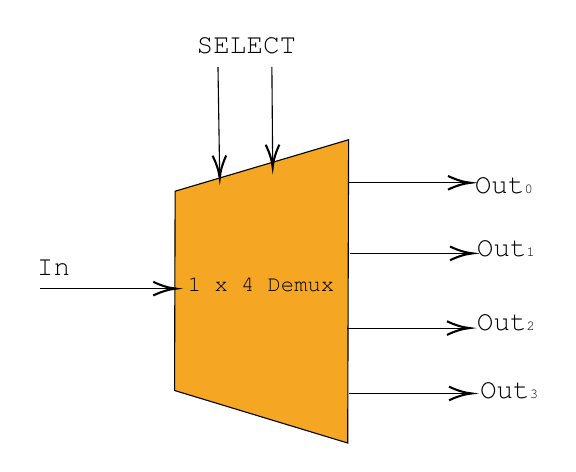
\begin{tikzpicture}[x=0.75pt,y=0.75pt,yscale=-1,xscale=1]
%uncomment if require: \path (0,300); %set diagram left start at 0, and has height of 300

%Shape: Trapezoid [id:dp8819284031411343] 
\draw  [fill={rgb, 255:red, 245; green, 166; blue, 35 }  ,fill opacity=1 ] (318.74,245.12) -- (235.32,219.82) -- (235.6,123.8) -- (319.18,99) -- cycle ;
%Straight Lines [id:da3811016173438192] 
\draw    (319,119.75) -- (376,119.75) ;
\draw [shift={(378,119.75)}, rotate = 180] [color={rgb, 255:red, 0; green, 0; blue, 0 }  ][line width=0.75]    (10.93,-3.29) .. controls (6.95,-1.4) and (3.31,-0.3) .. (0,0) .. controls (3.31,0.3) and (6.95,1.4) .. (10.93,3.29)   ;
%Straight Lines [id:da3695279660393864] 
\draw    (170.5,170.75) -- (234,170.75) ;
\draw [shift={(236,170.75)}, rotate = 180] [color={rgb, 255:red, 0; green, 0; blue, 0 }  ][line width=0.75]    (10.93,-3.29) .. controls (6.95,-1.4) and (3.31,-0.3) .. (0,0) .. controls (3.31,0.3) and (6.95,1.4) .. (10.93,3.29)   ;
%Straight Lines [id:da8955779809256085] 
\draw    (282.21,63.89) -- (282.59,110.33) ;
\draw [shift={(282.61,112.33)}, rotate = 269.53] [color={rgb, 255:red, 0; green, 0; blue, 0 }  ][line width=0.75]    (10.93,-3.29) .. controls (6.95,-1.4) and (3.31,-0.3) .. (0,0) .. controls (3.31,0.3) and (6.95,1.4) .. (10.93,3.29)   ;
%Straight Lines [id:da2688029751798525] 
\draw    (256.24,63.89) -- (257.05,115.58) ;
\draw [shift={(257.09,117.58)}, rotate = 269.1] [color={rgb, 255:red, 0; green, 0; blue, 0 }  ][line width=0.75]    (10.93,-3.29) .. controls (6.95,-1.4) and (3.31,-0.3) .. (0,0) .. controls (3.31,0.3) and (6.95,1.4) .. (10.93,3.29)   ;
%Straight Lines [id:da3254374593013373] 
\draw    (320,153.75) -- (377,153.75) ;
\draw [shift={(379,153.75)}, rotate = 180] [color={rgb, 255:red, 0; green, 0; blue, 0 }  ][line width=0.75]    (10.93,-3.29) .. controls (6.95,-1.4) and (3.31,-0.3) .. (0,0) .. controls (3.31,0.3) and (6.95,1.4) .. (10.93,3.29)   ;
%Straight Lines [id:da660432657953691] 
\draw    (318.5,189.75) -- (375.5,189.75) ;
\draw [shift={(377.5,189.75)}, rotate = 180] [color={rgb, 255:red, 0; green, 0; blue, 0 }  ][line width=0.75]    (10.93,-3.29) .. controls (6.95,-1.4) and (3.31,-0.3) .. (0,0) .. controls (3.31,0.3) and (6.95,1.4) .. (10.93,3.29)   ;
%Straight Lines [id:da8518268504183729] 
\draw    (319.5,221.25) -- (376.5,221.25) ;
\draw [shift={(378.5,221.25)}, rotate = 180] [color={rgb, 255:red, 0; green, 0; blue, 0 }  ][line width=0.75]    (10.93,-3.29) .. controls (6.95,-1.4) and (3.31,-0.3) .. (0,0) .. controls (3.31,0.3) and (6.95,1.4) .. (10.93,3.29)   ;

% Text Node
\draw (394,121) node   [align=left] {{\fontfamily{pcr}\selectfont Out{\tiny 0}}};
% Text Node
\draw (395,151.5) node   [align=left] {{\fontfamily{pcr}\selectfont Out{\tiny 1}}};
% Text Node
\draw (395,187) node   [align=left] {{\fontfamily{pcr}\selectfont Out{\tiny 2}}};
% Text Node
\draw (396.5,220) node   [align=left] {{\fontfamily{pcr}\selectfont Out{\tiny 3}}};
% Text Node
\draw (277,169) node   [align=left] {{\fontfamily{pcr}\selectfont {\footnotesize 1 x 4 Demux}}};
% Text Node
\draw (270,53.5) node   [align=left] {{\fontfamily{pcr}\selectfont SELECT}};
% Text Node
\draw (177,160.5) node   [align=left] {{\fontfamily{pcr}\selectfont In}};


\end{tikzpicture}

			\end{frame}
			
			\begin{frame}
             	\frametitle{Demultiplexer}
             	\begin{itemize}
             		\item Here's the actual logical circuit
             	\end{itemize}
             	\centering
             	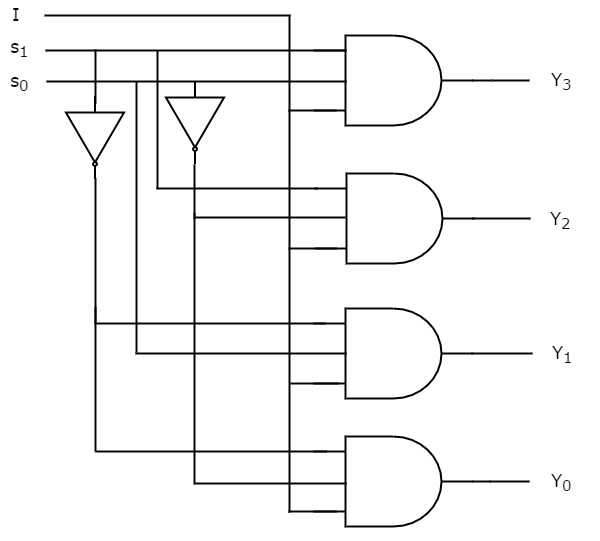
\includegraphics[width=0.6\textwidth]{demultiplexer}
             \end{frame}	
			
			
			% TODO Talk about math + applications in CPUs
			% TODO Talk about broader scope applications (???)
			% TODO Add a section to talk about project		             
             
        \subsection{Applications}
             
             \begin{frame}
                \vfill
                \centering
                \begin{beamercolorbox}[sep=8pt,center,shadow=true,rounded=true]{title}
                    \usebeamerfont{title}Applications\par%
                \end{beamercolorbox}
                \vfill
             \end{frame}
             
             \begin{frame}
             	\frametitle{Applications of Multiplexers}
             	\begin{itemize}
             		\item So how \textbf{useful} are these, anyway?
             		\item As it turns out, there are clear mathematical reasons why
             	\end{itemize}
             	
             \end{frame}
             
             \begin{frame}
             	\frametitle{Applications of Multiplexers}
             	\begin{itemize}
             		\item Consider the computer
             		\item CPUs need to leverage \textbf{muxes} and \textbf{demuxes} to process instructions and data efficiently
             		\item In particular, think of the ALU (what your projects have been, but way bigger)
             	\end{itemize}
             	
             \end{frame}
             
             
             \begin{frame}
             	\frametitle{Applications of Multiplexers}
             	\begin{itemize}
             		\item We provide them for you in the projects, but consider where the inputs for these ALU operations come from
             		\item If you think back to 216, the actual data comes from memory locations
             		\item To keep the math from becoming utter spaghetti, let's talk about \textbf{32-bit} systems for now.
             		
             	\end{itemize}
             	
             \end{frame}
             
             \begin{frame}
             
             	\frametitle{Applications of Multiplexers}
             	\begin{itemize}
             		\item Knowing that an ALU performs crucial operations that depend on the inputs it gets, let's figure out how we'd access those inputs
             		\item First of all, does anyone know how many memory addresses a 32-bit system would have?
             		
             	\end{itemize}
             	
             \end{frame}
             
             \begin{frame}
             
             	\frametitle{Applications of Multiplexers}
             	\begin{itemize}
             		\item Knowing that an ALU performs crucial operations that depend on the inputs it gets, let's figure out how we'd access those inputs
             		\item First of all, does anyone know how many memory addresses a 32-bit system would have? \newline
             		
             	\end{itemize}
             	
             	\centering
             	
             	\begin{Huge}
             		\texttt{$2^{32} = 4294967296$}
             	\end{Huge}
             	
             \end{frame}
             
             
             \begin{frame}
             
             	\frametitle{Applications of Multiplexers}
             	
             	\begin{itemize}
             		\item What would the inside of our computers be like if we had a little wire connecting each of those individual memory addresses to the ALU?
             	\end{itemize}
    
             	
             \end{frame}
             
             \begin{frame}
             	\frametitle{Applications of Multiplexers}
             	\centering
             	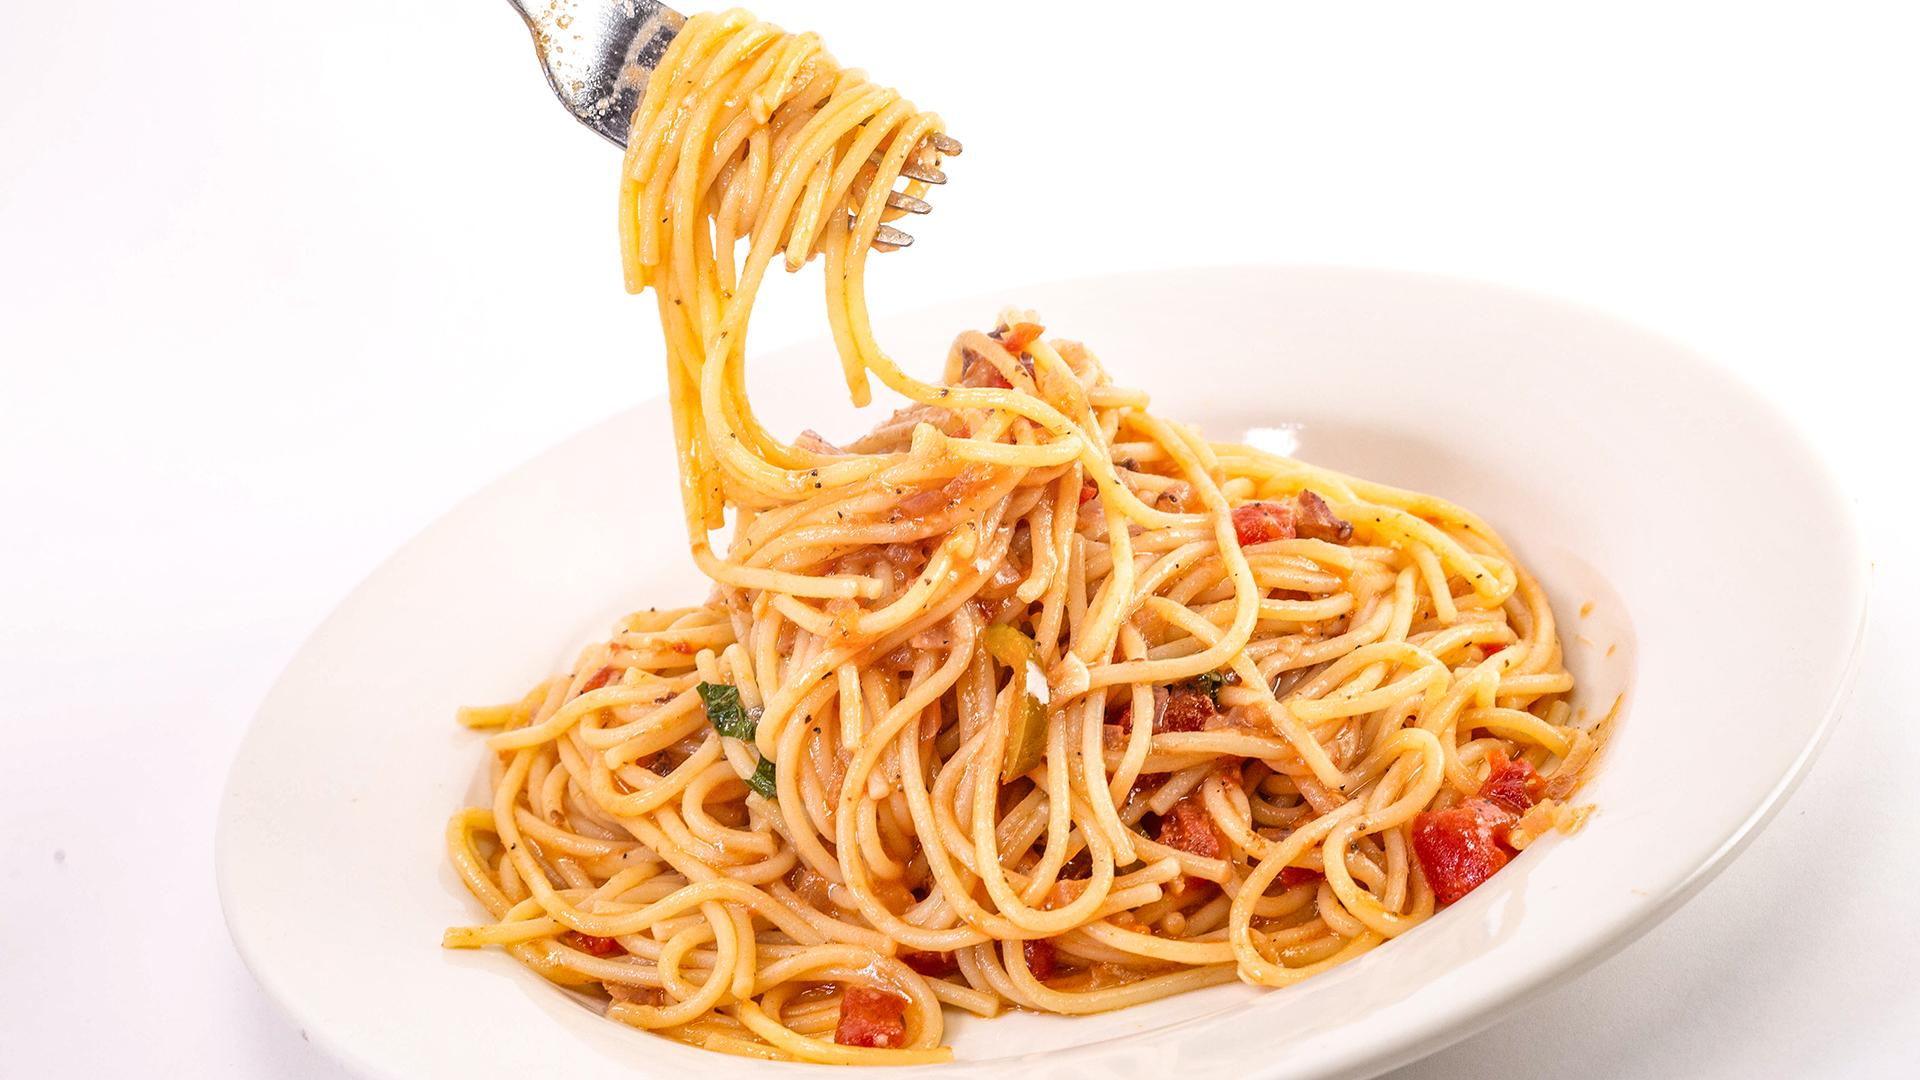
\includegraphics[width=0.9\textwidth]{spaghetti}
             \end{frame}
             
             \begin{frame}
             	\frametitle{Applications of Multiplexers}
             	\begin{itemize}
             		\item Instead of having around 4 million individual wires, we can use a multiplexer
             		\item How much would that cut us down to? (Remember, 32-bit architecture)
             	\end{itemize}
             \end{frame}
             
             
             \begin{frame}
             	\frametitle{Applications of Multiplexers}
             	\begin{itemize}
             		\item Instead of having around 4 million individual wires, we can use a multiplexer
             		\item How much would that cut us down to? (Remember, 32-bit architecture)
             		\item \textbf{We'd only need 1 output wire and 32 selector wires! (zoo wee mama)}
             		\item Keep in mind that modern ALUs can do way more than just add, subtract, and do simple logic gate operations, so this sort of implementation is majorly useful for us
             		\item P.S. How do you think it gets put back in memory?
             	\end{itemize}
             \end{frame}
             
             
             \begin{frame}
             	\frametitle{Applications of Multiplexers}
             	\begin{itemize}
             		\item Just food for thought- multiplexing and demultiplexing is hugely useful for us in other realms as well
             		\item How do you think phone calls are made on landlines? Is there really a wire that connects your landline to every other phone in the world?
             		\item Remember cable TV? (Emphasis on cable)
             		\item As it turns out, multiplexing and demultiplexing has proved very useful for us within the digital logic realm and outside of it
             	\end{itemize}
             \end{frame}
             
             
		\subsection{Project 4}
		
		
		\begin{frame}
                \vfill
                \centering
                \begin{beamercolorbox}[sep=8pt,center,shadow=true,rounded=true]{title}
                    \usebeamerfont{title}Project 4\par%
                \end{beamercolorbox}
                \vfill
             \end{frame}
             
             
   
   		
    
\end{document}
